\documentclass[twoside]{book}

% Packages required by doxygen
\usepackage{fixltx2e}
\usepackage{calc}
\usepackage{doxygen}
\usepackage[export]{adjustbox} % also loads graphicx
\usepackage{graphicx}
\usepackage[utf8]{inputenc}
\usepackage{makeidx}
\usepackage{multicol}
\usepackage{multirow}
\PassOptionsToPackage{warn}{textcomp}
\usepackage{textcomp}
\usepackage[nointegrals]{wasysym}
\usepackage[table]{xcolor}

% Font selection
\usepackage[T1]{fontenc}
\usepackage[scaled=.90]{helvet}
\usepackage{courier}
\usepackage{amssymb}
\usepackage{sectsty}
\renewcommand{\familydefault}{\sfdefault}
\allsectionsfont{%
  \fontseries{bc}\selectfont%
  \color{darkgray}%
}
\renewcommand{\DoxyLabelFont}{%
  \fontseries{bc}\selectfont%
  \color{darkgray}%
}
\newcommand{\+}{\discretionary{\mbox{\scriptsize$\hookleftarrow$}}{}{}}

% Page & text layout
\usepackage{geometry}
\geometry{%
  a4paper,%
  top=2.5cm,%
  bottom=2.5cm,%
  left=2.5cm,%
  right=2.5cm%
}
\tolerance=750
\hfuzz=15pt
\hbadness=750
\setlength{\emergencystretch}{15pt}
\setlength{\parindent}{0cm}
\setlength{\parskip}{3ex plus 2ex minus 2ex}
\makeatletter
\renewcommand{\paragraph}{%
  \@startsection{paragraph}{4}{0ex}{-1.0ex}{1.0ex}{%
    \normalfont\normalsize\bfseries\SS@parafont%
  }%
}
\renewcommand{\subparagraph}{%
  \@startsection{subparagraph}{5}{0ex}{-1.0ex}{1.0ex}{%
    \normalfont\normalsize\bfseries\SS@subparafont%
  }%
}
\makeatother

% Headers & footers
\usepackage{fancyhdr}
\pagestyle{fancyplain}
\fancyhead[LE]{\fancyplain{}{\bfseries\thepage}}
\fancyhead[CE]{\fancyplain{}{}}
\fancyhead[RE]{\fancyplain{}{\bfseries\leftmark}}
\fancyhead[LO]{\fancyplain{}{\bfseries\rightmark}}
\fancyhead[CO]{\fancyplain{}{}}
\fancyhead[RO]{\fancyplain{}{\bfseries\thepage}}
\fancyfoot[LE]{\fancyplain{}{}}
\fancyfoot[CE]{\fancyplain{}{}}
\fancyfoot[RE]{\fancyplain{}{\bfseries\scriptsize Generated by Doxygen }}
\fancyfoot[LO]{\fancyplain{}{\bfseries\scriptsize Generated by Doxygen }}
\fancyfoot[CO]{\fancyplain{}{}}
\fancyfoot[RO]{\fancyplain{}{}}
\renewcommand{\footrulewidth}{0.4pt}
\renewcommand{\chaptermark}[1]{%
  \markboth{#1}{}%
}
\renewcommand{\sectionmark}[1]{%
  \markright{\thesection\ #1}%
}

% Indices & bibliography
\usepackage{natbib}
\usepackage[titles]{tocloft}
\setcounter{tocdepth}{3}
\setcounter{secnumdepth}{5}
\makeindex

% Hyperlinks (required, but should be loaded last)
\usepackage{ifpdf}
\ifpdf
  \usepackage[pdftex,pagebackref=true]{hyperref}
\else
  \usepackage[ps2pdf,pagebackref=true]{hyperref}
\fi
\hypersetup{%
  colorlinks=true,%
  linkcolor=blue,%
  citecolor=blue,%
  unicode%
}

% Custom commands
\newcommand{\clearemptydoublepage}{%
  \newpage{\pagestyle{empty}\cleardoublepage}%
}

\usepackage{caption}
\captionsetup{labelsep=space,justification=centering,font={bf},singlelinecheck=off,skip=4pt,position=top}

%===== C O N T E N T S =====

\begin{document}

% Titlepage & ToC
\hypersetup{pageanchor=false,
             bookmarksnumbered=true,
             pdfencoding=unicode
            }
\pagenumbering{alph}
\begin{titlepage}
\vspace*{7cm}
\begin{center}%
{\Large My Proxy }\\
\vspace*{1cm}
{\large Generated by Doxygen 1.8.12}\\
\end{center}
\end{titlepage}
\clearemptydoublepage
\pagenumbering{roman}
\tableofcontents
\clearemptydoublepage
\pagenumbering{arabic}
\hypersetup{pageanchor=true}

%--- Begin generated contents ---
\chapter{docker-\/proxy}
\label{md__r_e_a_d_m_e}
\hypertarget{md__r_e_a_d_m_e}{}
docker proxy 
\chapter{Namespace Index}
\section{Namespace List}
Here is a list of all namespaces with brief descriptions\+:\begin{DoxyCompactList}
\item\contentsline{section}{\hyperlink{namespacedocker-proxy}{docker-\/proxy} }{\pageref{namespacedocker-proxy}}{}
\item\contentsline{section}{\hyperlink{namespacedocker-proxy_1_1config__parser}{docker-\/proxy.\+config\+\_\+parser} }{\pageref{namespacedocker-proxy_1_1config__parser}}{}
\item\contentsline{section}{\hyperlink{namespacedocker-proxy_1_1connect__docker__server}{docker-\/proxy.\+connect\+\_\+docker\+\_\+server} }{\pageref{namespacedocker-proxy_1_1connect__docker__server}}{}
\item\contentsline{section}{\hyperlink{namespacedocker-proxy_1_1models}{docker-\/proxy.\+models} }{\pageref{namespacedocker-proxy_1_1models}}{}
\item\contentsline{section}{\hyperlink{namespacedocker-proxy_1_1my__proxy}{docker-\/proxy.\+my\+\_\+proxy} }{\pageref{namespacedocker-proxy_1_1my__proxy}}{}
\item\contentsline{section}{\hyperlink{namespacedocker-proxy_1_1unit__tests}{docker-\/proxy.\+unit\+\_\+tests} }{\pageref{namespacedocker-proxy_1_1unit__tests}}{}
\item\contentsline{section}{\hyperlink{namespacedocker-proxy_1_1validate__hostname}{docker-\/proxy.\+validate\+\_\+hostname} }{\pageref{namespacedocker-proxy_1_1validate__hostname}}{}
\end{DoxyCompactList}

\chapter{Hierarchical Index}
\section{Class Hierarchy}
This inheritance list is sorted roughly, but not completely, alphabetically\+:\begin{DoxyCompactList}
\item Exception\begin{DoxyCompactList}
\item \contentsline{section}{docker-\/proxy.my\+\_\+proxy.\+Invalid\+Usage}{\pageref{classdocker-proxy_1_1my__proxy_1_1_invalid_usage}}{}
\end{DoxyCompactList}
\item Model\begin{DoxyCompactList}
\item \contentsline{section}{docker-\/proxy.models.\+Container\+Names}{\pageref{classdocker-proxy_1_1models_1_1_container_names}}{}
\item \contentsline{section}{docker-\/proxy.my\+\_\+proxy.\+Container\+Names}{\pageref{classdocker-proxy_1_1my__proxy_1_1_container_names}}{}
\item \contentsline{section}{docker-\/proxy.my\+\_\+proxy.\+Mount\+Points}{\pageref{classdocker-proxy_1_1my__proxy_1_1_mount_points}}{}
\end{DoxyCompactList}
\item Test\+Case\begin{DoxyCompactList}
\item \contentsline{section}{docker-\/proxy.unit\+\_\+tests.\+Md5\+Test}{\pageref{classdocker-proxy_1_1unit__tests_1_1_md5_test}}{}
\end{DoxyCompactList}
\end{DoxyCompactList}

\chapter{Class Index}
\section{Class List}
Here are the classes, structs, unions and interfaces with brief descriptions\+:\begin{DoxyCompactList}
\item\contentsline{section}{\hyperlink{classdocker-proxy_1_1models_1_1_container_names}{docker-\/proxy.\+models.\+Container\+Names} }{\pageref{classdocker-proxy_1_1models_1_1_container_names}}{}
\item\contentsline{section}{\hyperlink{classdocker-proxy_1_1my__proxy_1_1_container_names}{docker-\/proxy.\+my\+\_\+proxy.\+Container\+Names} }{\pageref{classdocker-proxy_1_1my__proxy_1_1_container_names}}{}
\item\contentsline{section}{\hyperlink{classdocker-proxy_1_1my__proxy_1_1_invalid_usage}{docker-\/proxy.\+my\+\_\+proxy.\+Invalid\+Usage} }{\pageref{classdocker-proxy_1_1my__proxy_1_1_invalid_usage}}{}
\item\contentsline{section}{\hyperlink{classdocker-proxy_1_1unit__tests_1_1_md5_test}{docker-\/proxy.\+unit\+\_\+tests.\+Md5\+Test} }{\pageref{classdocker-proxy_1_1unit__tests_1_1_md5_test}}{}
\item\contentsline{section}{\hyperlink{classdocker-proxy_1_1my__proxy_1_1_mount_points}{docker-\/proxy.\+my\+\_\+proxy.\+Mount\+Points} }{\pageref{classdocker-proxy_1_1my__proxy_1_1_mount_points}}{}
\end{DoxyCompactList}

\chapter{File Index}
\section{File List}
Here is a list of all files with brief descriptions\+:\begin{DoxyCompactList}
\item\contentsline{section}{\hyperlink{____init_____8py}{\+\_\+\+\_\+init\+\_\+\+\_\+.\+py} }{\pageref{____init_____8py}}{}
\item\contentsline{section}{\hyperlink{config__parser_8py}{config\+\_\+parser.\+py} }{\pageref{config__parser_8py}}{}
\item\contentsline{section}{\hyperlink{connect__docker__server_8py}{connect\+\_\+docker\+\_\+server.\+py} }{\pageref{connect__docker__server_8py}}{}
\item\contentsline{section}{\hyperlink{models_8py}{models.\+py} }{\pageref{models_8py}}{}
\item\contentsline{section}{\hyperlink{my__proxy_8py}{my\+\_\+proxy.\+py} }{\pageref{my__proxy_8py}}{}
\item\contentsline{section}{\hyperlink{unit__tests_8py}{unit\+\_\+tests.\+py} }{\pageref{unit__tests_8py}}{}
\item\contentsline{section}{\hyperlink{validate__hostname_8py}{validate\+\_\+hostname.\+py} }{\pageref{validate__hostname_8py}}{}
\end{DoxyCompactList}

\chapter{Namespace Documentation}
\hypertarget{namespacedocker-proxy}{}\section{docker-\/proxy Namespace Reference}
\label{namespacedocker-proxy}\index{docker-\/proxy@{docker-\/proxy}}
\subsection*{Namespaces}
\begin{DoxyCompactItemize}
\item 
 \hyperlink{namespacedocker-proxy_1_1config__parser}{config\+\_\+parser}
\item 
 \hyperlink{namespacedocker-proxy_1_1connect__docker__server}{connect\+\_\+docker\+\_\+server}
\item 
 \hyperlink{namespacedocker-proxy_1_1models}{models}
\item 
 \hyperlink{namespacedocker-proxy_1_1my__proxy}{my\+\_\+proxy}
\item 
 \hyperlink{namespacedocker-proxy_1_1unit__tests}{unit\+\_\+tests}
\item 
 \hyperlink{namespacedocker-proxy_1_1validate__hostname}{validate\+\_\+hostname}
\end{DoxyCompactItemize}
\subsection*{Variables}
\begin{DoxyCompactItemize}
\item 
\hyperlink{namespacedocker-proxy_a77b1cf15d8b7127338d8596c99d67ed7}{app} = Flask(\+\_\+\+\_\+name\+\_\+\+\_\+)
\end{DoxyCompactItemize}


\subsection{Variable Documentation}
\hypertarget{namespacedocker-proxy_a77b1cf15d8b7127338d8596c99d67ed7}{}\label{namespacedocker-proxy_a77b1cf15d8b7127338d8596c99d67ed7} 
\index{docker-\/proxy@{docker-\/proxy}!app@{app}}
\index{app@{app}!docker-\/proxy@{docker-\/proxy}}
\subsubsection{\texorpdfstring{app}{app}}
{\footnotesize\ttfamily docker-\/proxy.\+app = Flask(\+\_\+\+\_\+name\+\_\+\+\_\+)}



Definition at line 5 of file \+\_\+\+\_\+init\+\_\+\+\_\+.\+py.


\hypertarget{namespacedocker-proxy_1_1config__parser}{}\section{docker-\/proxy.config\+\_\+parser Namespace Reference}
\label{namespacedocker-proxy_1_1config__parser}\index{docker-\/proxy.\+config\+\_\+parser@{docker-\/proxy.\+config\+\_\+parser}}
\subsection*{Functions}
\begin{DoxyCompactItemize}
\item 
def \hyperlink{namespacedocker-proxy_1_1config__parser_aa9dfa23e3cb83a9b109517727216624a}{check\+\_\+if\+\_\+config\+\_\+exists} (config\+\_\+file)
\item 
def \hyperlink{namespacedocker-proxy_1_1config__parser_a52b3461dc4ed5a410f566197208b4b13}{config\+\_\+params} (section)
\end{DoxyCompactItemize}


\subsection{Function Documentation}
\hypertarget{namespacedocker-proxy_1_1config__parser_aa9dfa23e3cb83a9b109517727216624a}{}\label{namespacedocker-proxy_1_1config__parser_aa9dfa23e3cb83a9b109517727216624a} 
\index{docker-\/proxy\+::config\+\_\+parser@{docker-\/proxy\+::config\+\_\+parser}!check\+\_\+if\+\_\+config\+\_\+exists@{check\+\_\+if\+\_\+config\+\_\+exists}}
\index{check\+\_\+if\+\_\+config\+\_\+exists@{check\+\_\+if\+\_\+config\+\_\+exists}!docker-\/proxy\+::config\+\_\+parser@{docker-\/proxy\+::config\+\_\+parser}}
\subsubsection{\texorpdfstring{check\+\_\+if\+\_\+config\+\_\+exists()}{check\_if\_config\_exists()}}
{\footnotesize\ttfamily def docker-\/proxy.\+config\+\_\+parser.\+check\+\_\+if\+\_\+config\+\_\+exists (\begin{DoxyParamCaption}\item[{}]{config\+\_\+file }\end{DoxyParamCaption})}



Definition at line 6 of file config\+\_\+parser.\+py.

\hypertarget{namespacedocker-proxy_1_1config__parser_a52b3461dc4ed5a410f566197208b4b13}{}\label{namespacedocker-proxy_1_1config__parser_a52b3461dc4ed5a410f566197208b4b13} 
\index{docker-\/proxy\+::config\+\_\+parser@{docker-\/proxy\+::config\+\_\+parser}!config\+\_\+params@{config\+\_\+params}}
\index{config\+\_\+params@{config\+\_\+params}!docker-\/proxy\+::config\+\_\+parser@{docker-\/proxy\+::config\+\_\+parser}}
\subsubsection{\texorpdfstring{config\+\_\+params()}{config\_params()}}
{\footnotesize\ttfamily def docker-\/proxy.\+config\+\_\+parser.\+config\+\_\+params (\begin{DoxyParamCaption}\item[{}]{section }\end{DoxyParamCaption})}



Definition at line 15 of file config\+\_\+parser.\+py.


\hypertarget{namespacedocker-proxy_1_1connect__docker__server}{}\section{docker-\/proxy.connect\+\_\+docker\+\_\+server Namespace Reference}
\label{namespacedocker-proxy_1_1connect__docker__server}\index{docker-\/proxy.\+connect\+\_\+docker\+\_\+server@{docker-\/proxy.\+connect\+\_\+docker\+\_\+server}}
\subsection*{Functions}
\begin{DoxyCompactItemize}
\item 
def \hyperlink{namespacedocker-proxy_1_1connect__docker__server_a5a405d25b986678755c9a1aedeb066f8}{connect\+\_\+docker\+\_\+server} ()
\end{DoxyCompactItemize}
\subsection*{Variables}
\begin{DoxyCompactItemize}
\item 
def \hyperlink{namespacedocker-proxy_1_1connect__docker__server_aa7f3f87149d03ba3fd92b1b60a011454}{connect} = \hyperlink{namespacedocker-proxy_1_1connect__docker__server_a5a405d25b986678755c9a1aedeb066f8}{connect\+\_\+docker\+\_\+server}()
\end{DoxyCompactItemize}


\subsection{Function Documentation}
\hypertarget{namespacedocker-proxy_1_1connect__docker__server_a5a405d25b986678755c9a1aedeb066f8}{}\label{namespacedocker-proxy_1_1connect__docker__server_a5a405d25b986678755c9a1aedeb066f8} 
\index{docker-\/proxy\+::connect\+\_\+docker\+\_\+server@{docker-\/proxy\+::connect\+\_\+docker\+\_\+server}!connect\+\_\+docker\+\_\+server@{connect\+\_\+docker\+\_\+server}}
\index{connect\+\_\+docker\+\_\+server@{connect\+\_\+docker\+\_\+server}!docker-\/proxy\+::connect\+\_\+docker\+\_\+server@{docker-\/proxy\+::connect\+\_\+docker\+\_\+server}}
\subsubsection{\texorpdfstring{connect\+\_\+docker\+\_\+server()}{connect\_docker\_server()}}
{\footnotesize\ttfamily def docker-\/proxy.\+connect\+\_\+docker\+\_\+server.\+connect\+\_\+docker\+\_\+server (\begin{DoxyParamCaption}{ }\end{DoxyParamCaption})}



Definition at line 8 of file connect\+\_\+docker\+\_\+server.\+py.



\subsection{Variable Documentation}
\hypertarget{namespacedocker-proxy_1_1connect__docker__server_aa7f3f87149d03ba3fd92b1b60a011454}{}\label{namespacedocker-proxy_1_1connect__docker__server_aa7f3f87149d03ba3fd92b1b60a011454} 
\index{docker-\/proxy\+::connect\+\_\+docker\+\_\+server@{docker-\/proxy\+::connect\+\_\+docker\+\_\+server}!connect@{connect}}
\index{connect@{connect}!docker-\/proxy\+::connect\+\_\+docker\+\_\+server@{docker-\/proxy\+::connect\+\_\+docker\+\_\+server}}
\subsubsection{\texorpdfstring{connect}{connect}}
{\footnotesize\ttfamily def docker-\/proxy.\+connect\+\_\+docker\+\_\+server.\+connect = \hyperlink{namespacedocker-proxy_1_1connect__docker__server_a5a405d25b986678755c9a1aedeb066f8}{connect\+\_\+docker\+\_\+server}()}



Definition at line 18 of file connect\+\_\+docker\+\_\+server.\+py.


\hypertarget{namespacedocker-proxy_1_1models}{}\section{docker-\/proxy.models Namespace Reference}
\label{namespacedocker-proxy_1_1models}\index{docker-\/proxy.\+models@{docker-\/proxy.\+models}}
\subsection*{Classes}
\begin{DoxyCompactItemize}
\item 
class \hyperlink{classdocker-proxy_1_1models_1_1_container_names}{Container\+Names}
\end{DoxyCompactItemize}
\subsection*{Variables}
\begin{DoxyCompactItemize}
\item 
\hyperlink{namespacedocker-proxy_1_1models_a6d8a79afafa0fb31efaeda3e08b9a31d}{db} = S\+Q\+L\+Alchemy()
\end{DoxyCompactItemize}


\subsection{Variable Documentation}
\hypertarget{namespacedocker-proxy_1_1models_a6d8a79afafa0fb31efaeda3e08b9a31d}{}\label{namespacedocker-proxy_1_1models_a6d8a79afafa0fb31efaeda3e08b9a31d} 
\index{docker-\/proxy\+::models@{docker-\/proxy\+::models}!db@{db}}
\index{db@{db}!docker-\/proxy\+::models@{docker-\/proxy\+::models}}
\subsubsection{\texorpdfstring{db}{db}}
{\footnotesize\ttfamily docker-\/proxy.\+models.\+db = S\+Q\+L\+Alchemy()}



Definition at line 3 of file models.\+py.


\hypertarget{namespacedocker-proxy_1_1my__proxy}{}\section{docker-\/proxy.my\+\_\+proxy Namespace Reference}
\label{namespacedocker-proxy_1_1my__proxy}\index{docker-\/proxy.\+my\+\_\+proxy@{docker-\/proxy.\+my\+\_\+proxy}}
\subsection*{Classes}
\begin{DoxyCompactItemize}
\item 
class \hyperlink{classdocker-proxy_1_1my__proxy_1_1_container_names}{Container\+Names}
\item 
class \hyperlink{classdocker-proxy_1_1my__proxy_1_1_invalid_usage}{Invalid\+Usage}
\item 
class \hyperlink{classdocker-proxy_1_1my__proxy_1_1_mount_points}{Mount\+Points}
\end{DoxyCompactItemize}
\subsection*{Functions}
\begin{DoxyCompactItemize}
\item 
def \hyperlink{namespacedocker-proxy_1_1my__proxy_a0c927506d8346f17b620ac8e131174d0}{handle\+\_\+invalid\+\_\+usage} (error)
\item 
def \hyperlink{namespacedocker-proxy_1_1my__proxy_a219b29b5c79ad35297fb1f1deef275a3}{require\+\_\+appkey} (view\+\_\+function)
\item 
def \hyperlink{namespacedocker-proxy_1_1my__proxy_a0bf8985afda99ee825115bd5df0b6b40}{give\+\_\+me\+\_\+something\+\_\+unique} (name\+\_\+of\+\_\+container, hostname, owner, password, service\+\_\+name)
\item 
def \hyperlink{namespacedocker-proxy_1_1my__proxy_a32ea0c997fb4530822b84a6861f9666c}{give\+\_\+me\+\_\+mount\+\_\+point} (owner, size\+\_\+plan)
\item 
def \hyperlink{namespacedocker-proxy_1_1my__proxy_a7c16c9ad1dd493bd800fb0ccb04cfe32}{docker\+\_\+create} (name\+\_\+id, username, password, service, diskspace, image\+\_\+name, internal\+\_\+port, exec\+\_\+this)
\item 
def \hyperlink{namespacedocker-proxy_1_1my__proxy_a5c4e8ad5904fc41dc6e53312834445ae}{storage\+\_\+sum} ()
\item 
def \hyperlink{namespacedocker-proxy_1_1my__proxy_a2d2a47f5b69859690e7d948cbe5898a4}{storage} ()
\item 
def \hyperlink{namespacedocker-proxy_1_1my__proxy_ae108a533f8a3353f199f69883994c3cf}{stasts} (container\+\_\+id)
\item 
def \hyperlink{namespacedocker-proxy_1_1my__proxy_a96423469e4fe05cd336a8af7cb28d2ba}{management} (container\+\_\+id)
\item 
def \hyperlink{namespacedocker-proxy_1_1my__proxy_abf1a0936dc4dd14a5aaa78854c6583ce}{executecommands} (name\+\_\+id)
\item 
def \hyperlink{namespacedocker-proxy_1_1my__proxy_aaab4affe92f8974338caa10c0cf70c22}{makevm} (name\+\_\+id)
\item 
def \hyperlink{namespacedocker-proxy_1_1my__proxy_ad3276ec211f2fe107e03e4ed5e346df6}{version} ()
\item 
def \hyperlink{namespacedocker-proxy_1_1my__proxy_a7f6173c933a3e2e679eedb795386a08e}{query} (name)
\item 
def \hyperlink{namespacedocker-proxy_1_1my__proxy_a51d957f776d16e54de05b7034b113c1f}{investigate} (container\+\_\+id)
\item 
def \hyperlink{namespacedocker-proxy_1_1my__proxy_a84a1e1b9285c530fcd8b04177d08cdb3}{showstuff} ()
\end{DoxyCompactItemize}
\subsection*{Variables}
\begin{DoxyCompactItemize}
\item 
\hyperlink{namespacedocker-proxy_1_1my__proxy_a1316b64a06ccf8940bd886efa8d18660}{app} = Flask(\+\_\+\+\_\+name\+\_\+\+\_\+)
\item 
\hyperlink{namespacedocker-proxy_1_1my__proxy_a3cda0544280d27f01985434ab3efa4b3}{db} = S\+Q\+L\+Alchemy(\hyperlink{namespacedocker-proxy_1_1my__proxy_a1316b64a06ccf8940bd886efa8d18660}{app})
\item 
\hyperlink{namespacedocker-proxy_1_1my__proxy_a4cb4fb47e79c0c24a5b66136731a0b0c}{debug}
\end{DoxyCompactItemize}


\subsection{Function Documentation}
\hypertarget{namespacedocker-proxy_1_1my__proxy_a7c16c9ad1dd493bd800fb0ccb04cfe32}{}\label{namespacedocker-proxy_1_1my__proxy_a7c16c9ad1dd493bd800fb0ccb04cfe32} 
\index{docker-\/proxy\+::my\+\_\+proxy@{docker-\/proxy\+::my\+\_\+proxy}!docker\+\_\+create@{docker\+\_\+create}}
\index{docker\+\_\+create@{docker\+\_\+create}!docker-\/proxy\+::my\+\_\+proxy@{docker-\/proxy\+::my\+\_\+proxy}}
\subsubsection{\texorpdfstring{docker\+\_\+create()}{docker\_create()}}
{\footnotesize\ttfamily def docker-\/proxy.\+my\+\_\+proxy.\+docker\+\_\+create (\begin{DoxyParamCaption}\item[{}]{name\+\_\+id,  }\item[{}]{username,  }\item[{}]{password,  }\item[{}]{service,  }\item[{}]{diskspace,  }\item[{}]{image\+\_\+name,  }\item[{}]{internal\+\_\+port,  }\item[{}]{exec\+\_\+this }\end{DoxyParamCaption})}

\begin{DoxyVerb}this function will create the container
:rtype : object
:return:
\end{DoxyVerb}
 

Definition at line 195 of file my\+\_\+proxy.\+py.

\hypertarget{namespacedocker-proxy_1_1my__proxy_abf1a0936dc4dd14a5aaa78854c6583ce}{}\label{namespacedocker-proxy_1_1my__proxy_abf1a0936dc4dd14a5aaa78854c6583ce} 
\index{docker-\/proxy\+::my\+\_\+proxy@{docker-\/proxy\+::my\+\_\+proxy}!executecommands@{executecommands}}
\index{executecommands@{executecommands}!docker-\/proxy\+::my\+\_\+proxy@{docker-\/proxy\+::my\+\_\+proxy}}
\subsubsection{\texorpdfstring{executecommands()}{executecommands()}}
{\footnotesize\ttfamily def docker-\/proxy.\+my\+\_\+proxy.\+executecommands (\begin{DoxyParamCaption}\item[{}]{name\+\_\+id }\end{DoxyParamCaption})}

\begin{DoxyVerb}this function will execute commands on the container
curl -i -H "secretkey:1234" -H "Content-Type: application/json" -X POST -d
'{"command":"htpasswd -b -c /etc/nginx/.htpasswd test test"}' http://arisvm:5000/api/seedboxes/execute/rtorrent

:param name_id:
:return:
\end{DoxyVerb}
 

Definition at line 321 of file my\+\_\+proxy.\+py.

\hypertarget{namespacedocker-proxy_1_1my__proxy_a32ea0c997fb4530822b84a6861f9666c}{}\label{namespacedocker-proxy_1_1my__proxy_a32ea0c997fb4530822b84a6861f9666c} 
\index{docker-\/proxy\+::my\+\_\+proxy@{docker-\/proxy\+::my\+\_\+proxy}!give\+\_\+me\+\_\+mount\+\_\+point@{give\+\_\+me\+\_\+mount\+\_\+point}}
\index{give\+\_\+me\+\_\+mount\+\_\+point@{give\+\_\+me\+\_\+mount\+\_\+point}!docker-\/proxy\+::my\+\_\+proxy@{docker-\/proxy\+::my\+\_\+proxy}}
\subsubsection{\texorpdfstring{give\+\_\+me\+\_\+mount\+\_\+point()}{give\_me\_mount\_point()}}
{\footnotesize\ttfamily def docker-\/proxy.\+my\+\_\+proxy.\+give\+\_\+me\+\_\+mount\+\_\+point (\begin{DoxyParamCaption}\item[{}]{owner,  }\item[{}]{size\+\_\+plan }\end{DoxyParamCaption})}

\begin{DoxyVerb}this function will generate a shared tmpfs volume, the size should always be in M
let's insert mount points into table, user is unique, every user will have unique mount points
\end{DoxyVerb}
 

Definition at line 167 of file my\+\_\+proxy.\+py.

\hypertarget{namespacedocker-proxy_1_1my__proxy_a0bf8985afda99ee825115bd5df0b6b40}{}\label{namespacedocker-proxy_1_1my__proxy_a0bf8985afda99ee825115bd5df0b6b40} 
\index{docker-\/proxy\+::my\+\_\+proxy@{docker-\/proxy\+::my\+\_\+proxy}!give\+\_\+me\+\_\+something\+\_\+unique@{give\+\_\+me\+\_\+something\+\_\+unique}}
\index{give\+\_\+me\+\_\+something\+\_\+unique@{give\+\_\+me\+\_\+something\+\_\+unique}!docker-\/proxy\+::my\+\_\+proxy@{docker-\/proxy\+::my\+\_\+proxy}}
\subsubsection{\texorpdfstring{give\+\_\+me\+\_\+something\+\_\+unique()}{give\_me\_something\_unique()}}
{\footnotesize\ttfamily def docker-\/proxy.\+my\+\_\+proxy.\+give\+\_\+me\+\_\+something\+\_\+unique (\begin{DoxyParamCaption}\item[{}]{name\+\_\+of\+\_\+container,  }\item[{}]{hostname,  }\item[{}]{owner,  }\item[{}]{password,  }\item[{}]{service\+\_\+name }\end{DoxyParamCaption})}

\begin{DoxyVerb}let's generate random and unique port
:rtype : object
\end{DoxyVerb}
 

Definition at line 134 of file my\+\_\+proxy.\+py.

\hypertarget{namespacedocker-proxy_1_1my__proxy_a0c927506d8346f17b620ac8e131174d0}{}\label{namespacedocker-proxy_1_1my__proxy_a0c927506d8346f17b620ac8e131174d0} 
\index{docker-\/proxy\+::my\+\_\+proxy@{docker-\/proxy\+::my\+\_\+proxy}!handle\+\_\+invalid\+\_\+usage@{handle\+\_\+invalid\+\_\+usage}}
\index{handle\+\_\+invalid\+\_\+usage@{handle\+\_\+invalid\+\_\+usage}!docker-\/proxy\+::my\+\_\+proxy@{docker-\/proxy\+::my\+\_\+proxy}}
\subsubsection{\texorpdfstring{handle\+\_\+invalid\+\_\+usage()}{handle\_invalid\_usage()}}
{\footnotesize\ttfamily def docker-\/proxy.\+my\+\_\+proxy.\+handle\+\_\+invalid\+\_\+usage (\begin{DoxyParamCaption}\item[{}]{error }\end{DoxyParamCaption})}



Definition at line 48 of file my\+\_\+proxy.\+py.

\hypertarget{namespacedocker-proxy_1_1my__proxy_a51d957f776d16e54de05b7034b113c1f}{}\label{namespacedocker-proxy_1_1my__proxy_a51d957f776d16e54de05b7034b113c1f} 
\index{docker-\/proxy\+::my\+\_\+proxy@{docker-\/proxy\+::my\+\_\+proxy}!investigate@{investigate}}
\index{investigate@{investigate}!docker-\/proxy\+::my\+\_\+proxy@{docker-\/proxy\+::my\+\_\+proxy}}
\subsubsection{\texorpdfstring{investigate()}{investigate()}}
{\footnotesize\ttfamily def docker-\/proxy.\+my\+\_\+proxy.\+investigate (\begin{DoxyParamCaption}\item[{}]{container\+\_\+id }\end{DoxyParamCaption})}

\begin{DoxyVerb}investigare container, can be name or id
curl -H 'secretkey:1234' http://localhost:5000/api/seedboxes/investigate/83f1ee418bc4975c1a76bbffb96fb914caeb13c0cea5d44010e3
:return:
\end{DoxyVerb}
 

Definition at line 426 of file my\+\_\+proxy.\+py.

\hypertarget{namespacedocker-proxy_1_1my__proxy_aaab4affe92f8974338caa10c0cf70c22}{}\label{namespacedocker-proxy_1_1my__proxy_aaab4affe92f8974338caa10c0cf70c22} 
\index{docker-\/proxy\+::my\+\_\+proxy@{docker-\/proxy\+::my\+\_\+proxy}!makevm@{makevm}}
\index{makevm@{makevm}!docker-\/proxy\+::my\+\_\+proxy@{docker-\/proxy\+::my\+\_\+proxy}}
\subsubsection{\texorpdfstring{makevm()}{makevm()}}
{\footnotesize\ttfamily def docker-\/proxy.\+my\+\_\+proxy.\+makevm (\begin{DoxyParamCaption}\item[{}]{name\+\_\+id }\end{DoxyParamCaption})}

\begin{DoxyVerb}curl -i -H "secretkey:1234" -H "Content-Type: application/json" -X POST -d '{"username":"dan","password":
"123456789", "options": {"diskspace":"500m","service":"ssh"}}' http://localhost:5000/api/seedboxes/new/sshdan
this will create a container
we parse the json data and take username/password and we insert this into db
:param name_id:
:return:
\end{DoxyVerb}
 

Definition at line 343 of file my\+\_\+proxy.\+py.

\hypertarget{namespacedocker-proxy_1_1my__proxy_a96423469e4fe05cd336a8af7cb28d2ba}{}\label{namespacedocker-proxy_1_1my__proxy_a96423469e4fe05cd336a8af7cb28d2ba} 
\index{docker-\/proxy\+::my\+\_\+proxy@{docker-\/proxy\+::my\+\_\+proxy}!management@{management}}
\index{management@{management}!docker-\/proxy\+::my\+\_\+proxy@{docker-\/proxy\+::my\+\_\+proxy}}
\subsubsection{\texorpdfstring{management()}{management()}}
{\footnotesize\ttfamily def docker-\/proxy.\+my\+\_\+proxy.\+management (\begin{DoxyParamCaption}\item[{}]{container\+\_\+id }\end{DoxyParamCaption})}

\begin{DoxyVerb}this function will restart/stop/kill an instace
curl -i -H 'secretkey:1234' -H "Content-Type: application/json" -X POST -d
'{"action":"start" }' http://localhost:5000/api/seedboxes/management/b90ea5517564
:param container_id:
:param timeout:
:return:
\end{DoxyVerb}
 

Definition at line 285 of file my\+\_\+proxy.\+py.

\hypertarget{namespacedocker-proxy_1_1my__proxy_a7f6173c933a3e2e679eedb795386a08e}{}\label{namespacedocker-proxy_1_1my__proxy_a7f6173c933a3e2e679eedb795386a08e} 
\index{docker-\/proxy\+::my\+\_\+proxy@{docker-\/proxy\+::my\+\_\+proxy}!query@{query}}
\index{query@{query}!docker-\/proxy\+::my\+\_\+proxy@{docker-\/proxy\+::my\+\_\+proxy}}
\subsubsection{\texorpdfstring{query()}{query()}}
{\footnotesize\ttfamily def docker-\/proxy.\+my\+\_\+proxy.\+query (\begin{DoxyParamCaption}\item[{}]{name }\end{DoxyParamCaption})}

\begin{DoxyVerb}look in the containers db and return values
curl -i -H 'secretkey:1234'  http://localhost:5000/api/seedboxes/query/nginx
:return:
\end{DoxyVerb}
 

Definition at line 410 of file my\+\_\+proxy.\+py.

\hypertarget{namespacedocker-proxy_1_1my__proxy_a219b29b5c79ad35297fb1f1deef275a3}{}\label{namespacedocker-proxy_1_1my__proxy_a219b29b5c79ad35297fb1f1deef275a3} 
\index{docker-\/proxy\+::my\+\_\+proxy@{docker-\/proxy\+::my\+\_\+proxy}!require\+\_\+appkey@{require\+\_\+appkey}}
\index{require\+\_\+appkey@{require\+\_\+appkey}!docker-\/proxy\+::my\+\_\+proxy@{docker-\/proxy\+::my\+\_\+proxy}}
\subsubsection{\texorpdfstring{require\+\_\+appkey()}{require\_appkey()}}
{\footnotesize\ttfamily def docker-\/proxy.\+my\+\_\+proxy.\+require\+\_\+appkey (\begin{DoxyParamCaption}\item[{}]{view\+\_\+function }\end{DoxyParamCaption})}

\begin{DoxyVerb}simple appkey validation
it will check presence of the header secretkey with value 123
:param view_function:
:return:
\end{DoxyVerb}
 

Definition at line 54 of file my\+\_\+proxy.\+py.

\hypertarget{namespacedocker-proxy_1_1my__proxy_a84a1e1b9285c530fcd8b04177d08cdb3}{}\label{namespacedocker-proxy_1_1my__proxy_a84a1e1b9285c530fcd8b04177d08cdb3} 
\index{docker-\/proxy\+::my\+\_\+proxy@{docker-\/proxy\+::my\+\_\+proxy}!showstuff@{showstuff}}
\index{showstuff@{showstuff}!docker-\/proxy\+::my\+\_\+proxy@{docker-\/proxy\+::my\+\_\+proxy}}
\subsubsection{\texorpdfstring{showstuff()}{showstuff()}}
{\footnotesize\ttfamily def docker-\/proxy.\+my\+\_\+proxy.\+showstuff (\begin{DoxyParamCaption}{ }\end{DoxyParamCaption})}

\begin{DoxyVerb}this will return all instances of a specific user
curl -H 'secretkey:1234' http://localhost:5000/api/seedboxes/showinstances?name_id=dan
:return:
\end{DoxyVerb}
 

Definition at line 443 of file my\+\_\+proxy.\+py.

\hypertarget{namespacedocker-proxy_1_1my__proxy_ae108a533f8a3353f199f69883994c3cf}{}\label{namespacedocker-proxy_1_1my__proxy_ae108a533f8a3353f199f69883994c3cf} 
\index{docker-\/proxy\+::my\+\_\+proxy@{docker-\/proxy\+::my\+\_\+proxy}!stasts@{stasts}}
\index{stasts@{stasts}!docker-\/proxy\+::my\+\_\+proxy@{docker-\/proxy\+::my\+\_\+proxy}}
\subsubsection{\texorpdfstring{stasts()}{stasts()}}
{\footnotesize\ttfamily def docker-\/proxy.\+my\+\_\+proxy.\+stasts (\begin{DoxyParamCaption}\item[{}]{container\+\_\+id }\end{DoxyParamCaption})}

\begin{DoxyVerb}get statistics from container
curl -i -H 'secretkey:1234'  http://localhost:5000/api/seedboxes/stats/vm6690_ssh
:param container_id:
:return:
\end{DoxyVerb}
 

Definition at line 268 of file my\+\_\+proxy.\+py.

\hypertarget{namespacedocker-proxy_1_1my__proxy_a2d2a47f5b69859690e7d948cbe5898a4}{}\label{namespacedocker-proxy_1_1my__proxy_a2d2a47f5b69859690e7d948cbe5898a4} 
\index{docker-\/proxy\+::my\+\_\+proxy@{docker-\/proxy\+::my\+\_\+proxy}!storage@{storage}}
\index{storage@{storage}!docker-\/proxy\+::my\+\_\+proxy@{docker-\/proxy\+::my\+\_\+proxy}}
\subsubsection{\texorpdfstring{storage()}{storage()}}
{\footnotesize\ttfamily def docker-\/proxy.\+my\+\_\+proxy.\+storage (\begin{DoxyParamCaption}{ }\end{DoxyParamCaption})}

\begin{DoxyVerb}curl -i -H "secretkey:1234" http://localhost:5000/api/seedboxes/storage
retunr alocated storage from db
:return:
\end{DoxyVerb}
 

Definition at line 255 of file my\+\_\+proxy.\+py.

\hypertarget{namespacedocker-proxy_1_1my__proxy_a5c4e8ad5904fc41dc6e53312834445ae}{}\label{namespacedocker-proxy_1_1my__proxy_a5c4e8ad5904fc41dc6e53312834445ae} 
\index{docker-\/proxy\+::my\+\_\+proxy@{docker-\/proxy\+::my\+\_\+proxy}!storage\+\_\+sum@{storage\+\_\+sum}}
\index{storage\+\_\+sum@{storage\+\_\+sum}!docker-\/proxy\+::my\+\_\+proxy@{docker-\/proxy\+::my\+\_\+proxy}}
\subsubsection{\texorpdfstring{storage\+\_\+sum()}{storage\_sum()}}
{\footnotesize\ttfamily def docker-\/proxy.\+my\+\_\+proxy.\+storage\+\_\+sum (\begin{DoxyParamCaption}{ }\end{DoxyParamCaption})}

\begin{DoxyVerb}function to check storage
:return:
\end{DoxyVerb}
 

Definition at line 242 of file my\+\_\+proxy.\+py.

\hypertarget{namespacedocker-proxy_1_1my__proxy_ad3276ec211f2fe107e03e4ed5e346df6}{}\label{namespacedocker-proxy_1_1my__proxy_ad3276ec211f2fe107e03e4ed5e346df6} 
\index{docker-\/proxy\+::my\+\_\+proxy@{docker-\/proxy\+::my\+\_\+proxy}!version@{version}}
\index{version@{version}!docker-\/proxy\+::my\+\_\+proxy@{docker-\/proxy\+::my\+\_\+proxy}}
\subsubsection{\texorpdfstring{version()}{version()}}
{\footnotesize\ttfamily def docker-\/proxy.\+my\+\_\+proxy.\+version (\begin{DoxyParamCaption}{ }\end{DoxyParamCaption})}

\begin{DoxyVerb}return versios of docker, used for whatever
:return:
\end{DoxyVerb}
 

Definition at line 395 of file my\+\_\+proxy.\+py.



\subsection{Variable Documentation}
\hypertarget{namespacedocker-proxy_1_1my__proxy_a1316b64a06ccf8940bd886efa8d18660}{}\label{namespacedocker-proxy_1_1my__proxy_a1316b64a06ccf8940bd886efa8d18660} 
\index{docker-\/proxy\+::my\+\_\+proxy@{docker-\/proxy\+::my\+\_\+proxy}!app@{app}}
\index{app@{app}!docker-\/proxy\+::my\+\_\+proxy@{docker-\/proxy\+::my\+\_\+proxy}}
\subsubsection{\texorpdfstring{app}{app}}
{\footnotesize\ttfamily docker-\/proxy.\+my\+\_\+proxy.\+app = Flask(\+\_\+\+\_\+name\+\_\+\+\_\+)}



Definition at line 18 of file my\+\_\+proxy.\+py.

\hypertarget{namespacedocker-proxy_1_1my__proxy_a3cda0544280d27f01985434ab3efa4b3}{}\label{namespacedocker-proxy_1_1my__proxy_a3cda0544280d27f01985434ab3efa4b3} 
\index{docker-\/proxy\+::my\+\_\+proxy@{docker-\/proxy\+::my\+\_\+proxy}!db@{db}}
\index{db@{db}!docker-\/proxy\+::my\+\_\+proxy@{docker-\/proxy\+::my\+\_\+proxy}}
\subsubsection{\texorpdfstring{db}{db}}
{\footnotesize\ttfamily docker-\/proxy.\+my\+\_\+proxy.\+db = S\+Q\+L\+Alchemy(\hyperlink{namespacedocker-proxy_1_1my__proxy_a1316b64a06ccf8940bd886efa8d18660}{app})}



Definition at line 25 of file my\+\_\+proxy.\+py.

\hypertarget{namespacedocker-proxy_1_1my__proxy_a4cb4fb47e79c0c24a5b66136731a0b0c}{}\label{namespacedocker-proxy_1_1my__proxy_a4cb4fb47e79c0c24a5b66136731a0b0c} 
\index{docker-\/proxy\+::my\+\_\+proxy@{docker-\/proxy\+::my\+\_\+proxy}!debug@{debug}}
\index{debug@{debug}!docker-\/proxy\+::my\+\_\+proxy@{docker-\/proxy\+::my\+\_\+proxy}}
\subsubsection{\texorpdfstring{debug}{debug}}
{\footnotesize\ttfamily docker-\/proxy.\+my\+\_\+proxy.\+debug}



Definition at line 459 of file my\+\_\+proxy.\+py.


\hypertarget{namespacedocker-proxy_1_1unit__tests}{}\section{docker-\/proxy.unit\+\_\+tests Namespace Reference}
\label{namespacedocker-proxy_1_1unit__tests}\index{docker-\/proxy.\+unit\+\_\+tests@{docker-\/proxy.\+unit\+\_\+tests}}
\subsection*{Classes}
\begin{DoxyCompactItemize}
\item 
class \hyperlink{classdocker-proxy_1_1unit__tests_1_1_md5_test}{Md5\+Test}
\end{DoxyCompactItemize}

\hypertarget{namespacedocker-proxy_1_1validate__hostname}{}\section{docker-\/proxy.validate\+\_\+hostname Namespace Reference}
\label{namespacedocker-proxy_1_1validate__hostname}\index{docker-\/proxy.\+validate\+\_\+hostname@{docker-\/proxy.\+validate\+\_\+hostname}}
\subsection*{Functions}
\begin{DoxyCompactItemize}
\item 
def \hyperlink{namespacedocker-proxy_1_1validate__hostname_a78870bf36758d0abb57f63eea91fd8b7}{isvalidhostname} (hostname)
\end{DoxyCompactItemize}


\subsection{Function Documentation}
\hypertarget{namespacedocker-proxy_1_1validate__hostname_a78870bf36758d0abb57f63eea91fd8b7}{}\label{namespacedocker-proxy_1_1validate__hostname_a78870bf36758d0abb57f63eea91fd8b7} 
\index{docker-\/proxy\+::validate\+\_\+hostname@{docker-\/proxy\+::validate\+\_\+hostname}!isvalidhostname@{isvalidhostname}}
\index{isvalidhostname@{isvalidhostname}!docker-\/proxy\+::validate\+\_\+hostname@{docker-\/proxy\+::validate\+\_\+hostname}}
\subsubsection{\texorpdfstring{isvalidhostname()}{isvalidhostname()}}
{\footnotesize\ttfamily def docker-\/proxy.\+validate\+\_\+hostname.\+isvalidhostname (\begin{DoxyParamCaption}\item[{}]{hostname }\end{DoxyParamCaption})}

\begin{DoxyVerb}this function will validate if hostname is valid
:param hostname:
:return:
\end{DoxyVerb}
 

Definition at line 5 of file validate\+\_\+hostname.\+py.


\chapter{Class Documentation}
\hypertarget{classdocker-proxy_1_1models_1_1_container_names}{}\section{docker-\/proxy.models.\+Container\+Names Class Reference}
\label{classdocker-proxy_1_1models_1_1_container_names}\index{docker-\/proxy.\+models.\+Container\+Names@{docker-\/proxy.\+models.\+Container\+Names}}
Inheritance diagram for docker-\/proxy.models.\+Container\+Names\+:\begin{figure}[H]
\begin{center}
\leavevmode
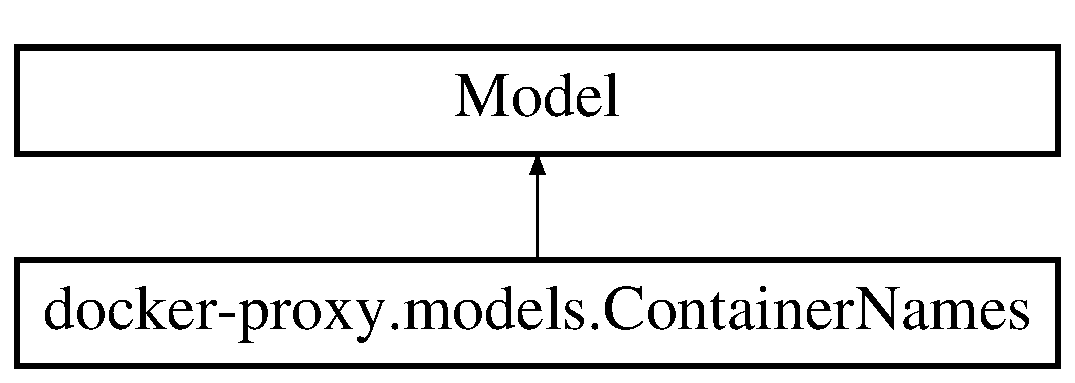
\includegraphics[height=2.000000cm]{classdocker-proxy_1_1models_1_1_container_names}
\end{center}
\end{figure}
\subsection*{Public Member Functions}
\begin{DoxyCompactItemize}
\item 
def \hyperlink{classdocker-proxy_1_1models_1_1_container_names_a51208829bf52ae24f5cf5891f486731b}{\+\_\+\+\_\+init\+\_\+\+\_\+} (self, \hyperlink{classdocker-proxy_1_1models_1_1_container_names_a6600e5199beb00fa24ff7b6b104cf4c1}{id}, \hyperlink{classdocker-proxy_1_1models_1_1_container_names_ae84f0bb3f85f0483fdbe500c78ca814f}{name\+\_\+of\+\_\+container})
\item 
def \hyperlink{classdocker-proxy_1_1models_1_1_container_names_a2b52c32297b1bb19f73687c9b21e5e50}{\+\_\+\+\_\+repr\+\_\+\+\_\+} (self)
\end{DoxyCompactItemize}
\subsection*{Static Public Attributes}
\begin{DoxyCompactItemize}
\item 
\hyperlink{classdocker-proxy_1_1models_1_1_container_names_a6600e5199beb00fa24ff7b6b104cf4c1}{id} = db.\+Column(db.\+Integer, primary\+\_\+key=True)
\item 
\hyperlink{classdocker-proxy_1_1models_1_1_container_names_ae84f0bb3f85f0483fdbe500c78ca814f}{name\+\_\+of\+\_\+container} = db.\+Column(db.\+String(80), unique=True)
\end{DoxyCompactItemize}


\subsection{Detailed Description}


Definition at line 5 of file models.\+py.



\subsection{Constructor \& Destructor Documentation}
\hypertarget{classdocker-proxy_1_1models_1_1_container_names_a51208829bf52ae24f5cf5891f486731b}{}\label{classdocker-proxy_1_1models_1_1_container_names_a51208829bf52ae24f5cf5891f486731b} 
\index{docker-\/proxy\+::models\+::\+Container\+Names@{docker-\/proxy\+::models\+::\+Container\+Names}!\+\_\+\+\_\+init\+\_\+\+\_\+@{\+\_\+\+\_\+init\+\_\+\+\_\+}}
\index{\+\_\+\+\_\+init\+\_\+\+\_\+@{\+\_\+\+\_\+init\+\_\+\+\_\+}!docker-\/proxy\+::models\+::\+Container\+Names@{docker-\/proxy\+::models\+::\+Container\+Names}}
\subsubsection{\texorpdfstring{\+\_\+\+\_\+init\+\_\+\+\_\+()}{\_\_init\_\_()}}
{\footnotesize\ttfamily def docker-\/proxy.\+models.\+Container\+Names.\+\_\+\+\_\+init\+\_\+\+\_\+ (\begin{DoxyParamCaption}\item[{}]{self,  }\item[{}]{id,  }\item[{}]{name\+\_\+of\+\_\+container }\end{DoxyParamCaption})}



Definition at line 10 of file models.\+py.



\subsection{Member Function Documentation}
\hypertarget{classdocker-proxy_1_1models_1_1_container_names_a2b52c32297b1bb19f73687c9b21e5e50}{}\label{classdocker-proxy_1_1models_1_1_container_names_a2b52c32297b1bb19f73687c9b21e5e50} 
\index{docker-\/proxy\+::models\+::\+Container\+Names@{docker-\/proxy\+::models\+::\+Container\+Names}!\+\_\+\+\_\+repr\+\_\+\+\_\+@{\+\_\+\+\_\+repr\+\_\+\+\_\+}}
\index{\+\_\+\+\_\+repr\+\_\+\+\_\+@{\+\_\+\+\_\+repr\+\_\+\+\_\+}!docker-\/proxy\+::models\+::\+Container\+Names@{docker-\/proxy\+::models\+::\+Container\+Names}}
\subsubsection{\texorpdfstring{\+\_\+\+\_\+repr\+\_\+\+\_\+()}{\_\_repr\_\_()}}
{\footnotesize\ttfamily def docker-\/proxy.\+models.\+Container\+Names.\+\_\+\+\_\+repr\+\_\+\+\_\+ (\begin{DoxyParamCaption}\item[{}]{self }\end{DoxyParamCaption})}



Definition at line 14 of file models.\+py.



\subsection{Member Data Documentation}
\hypertarget{classdocker-proxy_1_1models_1_1_container_names_a6600e5199beb00fa24ff7b6b104cf4c1}{}\label{classdocker-proxy_1_1models_1_1_container_names_a6600e5199beb00fa24ff7b6b104cf4c1} 
\index{docker-\/proxy\+::models\+::\+Container\+Names@{docker-\/proxy\+::models\+::\+Container\+Names}!id@{id}}
\index{id@{id}!docker-\/proxy\+::models\+::\+Container\+Names@{docker-\/proxy\+::models\+::\+Container\+Names}}
\subsubsection{\texorpdfstring{id}{id}}
{\footnotesize\ttfamily docker-\/proxy.\+models.\+Container\+Names.\+id = db.\+Column(db.\+Integer, primary\+\_\+key=True)\hspace{0.3cm}{\ttfamily [static]}}



Definition at line 7 of file models.\+py.

\hypertarget{classdocker-proxy_1_1models_1_1_container_names_ae84f0bb3f85f0483fdbe500c78ca814f}{}\label{classdocker-proxy_1_1models_1_1_container_names_ae84f0bb3f85f0483fdbe500c78ca814f} 
\index{docker-\/proxy\+::models\+::\+Container\+Names@{docker-\/proxy\+::models\+::\+Container\+Names}!name\+\_\+of\+\_\+container@{name\+\_\+of\+\_\+container}}
\index{name\+\_\+of\+\_\+container@{name\+\_\+of\+\_\+container}!docker-\/proxy\+::models\+::\+Container\+Names@{docker-\/proxy\+::models\+::\+Container\+Names}}
\subsubsection{\texorpdfstring{name\+\_\+of\+\_\+container}{name\_of\_container}}
{\footnotesize\ttfamily docker-\/proxy.\+models.\+Container\+Names.\+name\+\_\+of\+\_\+container = db.\+Column(db.\+String(80), unique=True)\hspace{0.3cm}{\ttfamily [static]}}



Definition at line 8 of file models.\+py.



The documentation for this class was generated from the following file\+:\begin{DoxyCompactItemize}
\item 
\hyperlink{models_8py}{models.\+py}\end{DoxyCompactItemize}

\hypertarget{classdocker-proxy_1_1my__proxy_1_1_container_names}{}\section{docker-\/proxy.my\+\_\+proxy.\+Container\+Names Class Reference}
\label{classdocker-proxy_1_1my__proxy_1_1_container_names}\index{docker-\/proxy.\+my\+\_\+proxy.\+Container\+Names@{docker-\/proxy.\+my\+\_\+proxy.\+Container\+Names}}
Inheritance diagram for docker-\/proxy.my\+\_\+proxy.\+Container\+Names\+:\begin{figure}[H]
\begin{center}
\leavevmode
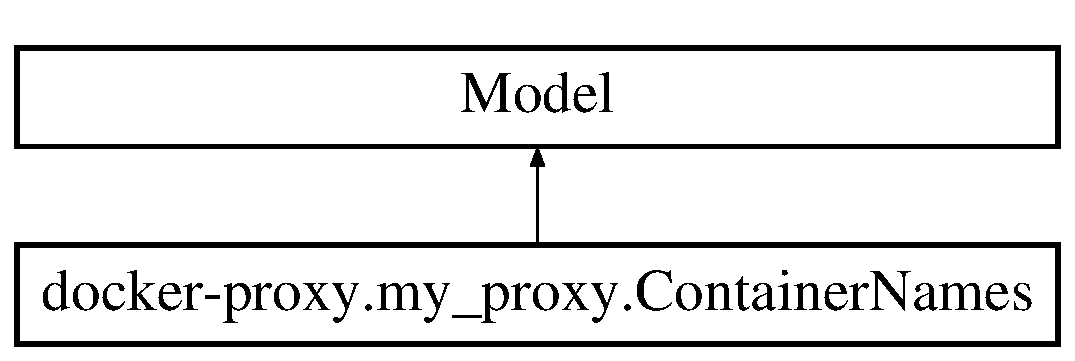
\includegraphics[height=2.000000cm]{classdocker-proxy_1_1my__proxy_1_1_container_names}
\end{center}
\end{figure}
\subsection*{Public Member Functions}
\begin{DoxyCompactItemize}
\item 
def \hyperlink{classdocker-proxy_1_1my__proxy_1_1_container_names_a6f793b87c5c96d4c3c8becfbc748ada9}{\+\_\+\+\_\+init\+\_\+\+\_\+} (self, \hyperlink{classdocker-proxy_1_1my__proxy_1_1_container_names_a5223d4e116bb162d327af3fbdf406c62}{name\+\_\+of\+\_\+container}, \hyperlink{classdocker-proxy_1_1my__proxy_1_1_container_names_aacca73fd2984a6225ff6f82fb681a508}{hostname}, \hyperlink{classdocker-proxy_1_1my__proxy_1_1_container_names_a18b80021fc434e7dac00f009f7a451b5}{owner}, \hyperlink{classdocker-proxy_1_1my__proxy_1_1_container_names_a5728904cb244540aa3421e07dc14cc84}{password}, \hyperlink{classdocker-proxy_1_1my__proxy_1_1_container_names_accfbd6e258c7ede9ac75360c54086e2a}{public\+\_\+port}, \hyperlink{classdocker-proxy_1_1my__proxy_1_1_container_names_ac067fae0674728a7064586300ef6b107}{service\+\_\+name})
\item 
def \hyperlink{classdocker-proxy_1_1my__proxy_1_1_container_names_a5bade0263a94bbfc7ffba0b4179ae27e}{\+\_\+\+\_\+repr\+\_\+\+\_\+} (self)
\end{DoxyCompactItemize}
\subsection*{Static Public Attributes}
\begin{DoxyCompactItemize}
\item 
\hyperlink{classdocker-proxy_1_1my__proxy_1_1_container_names_a7013f7adde5d40aedd4169afb3be1978}{id} = db.\+Column(db.\+Integer, primary\+\_\+key=True, autoincrement=True)
\item 
\hyperlink{classdocker-proxy_1_1my__proxy_1_1_container_names_a5223d4e116bb162d327af3fbdf406c62}{name\+\_\+of\+\_\+container} = db.\+Column(db.\+String(80), unique=True)
\item 
\hyperlink{classdocker-proxy_1_1my__proxy_1_1_container_names_aacca73fd2984a6225ff6f82fb681a508}{hostname} = db.\+Column(db.\+String(80))
\item 
\hyperlink{classdocker-proxy_1_1my__proxy_1_1_container_names_a18b80021fc434e7dac00f009f7a451b5}{owner} = db.\+Column(db.\+String(100))
\item 
\hyperlink{classdocker-proxy_1_1my__proxy_1_1_container_names_a5728904cb244540aa3421e07dc14cc84}{password} = db.\+Column(db.\+String(200))
\item 
\hyperlink{classdocker-proxy_1_1my__proxy_1_1_container_names_accfbd6e258c7ede9ac75360c54086e2a}{public\+\_\+port} = db.\+Column(db.\+Integer, unique=True)
\item 
\hyperlink{classdocker-proxy_1_1my__proxy_1_1_container_names_ac067fae0674728a7064586300ef6b107}{service\+\_\+name} = db.\+Column(db.\+String(100))
\end{DoxyCompactItemize}


\subsection{Detailed Description}
\begin{DoxyVerb}let's do ContainerNames tables
\end{DoxyVerb}
 

Definition at line 96 of file my\+\_\+proxy.\+py.



\subsection{Constructor \& Destructor Documentation}
\hypertarget{classdocker-proxy_1_1my__proxy_1_1_container_names_a6f793b87c5c96d4c3c8becfbc748ada9}{}\label{classdocker-proxy_1_1my__proxy_1_1_container_names_a6f793b87c5c96d4c3c8becfbc748ada9} 
\index{docker-\/proxy\+::my\+\_\+proxy\+::\+Container\+Names@{docker-\/proxy\+::my\+\_\+proxy\+::\+Container\+Names}!\+\_\+\+\_\+init\+\_\+\+\_\+@{\+\_\+\+\_\+init\+\_\+\+\_\+}}
\index{\+\_\+\+\_\+init\+\_\+\+\_\+@{\+\_\+\+\_\+init\+\_\+\+\_\+}!docker-\/proxy\+::my\+\_\+proxy\+::\+Container\+Names@{docker-\/proxy\+::my\+\_\+proxy\+::\+Container\+Names}}
\subsubsection{\texorpdfstring{\+\_\+\+\_\+init\+\_\+\+\_\+()}{\_\_init\_\_()}}
{\footnotesize\ttfamily def docker-\/proxy.\+my\+\_\+proxy.\+Container\+Names.\+\_\+\+\_\+init\+\_\+\+\_\+ (\begin{DoxyParamCaption}\item[{}]{self,  }\item[{}]{name\+\_\+of\+\_\+container,  }\item[{}]{hostname,  }\item[{}]{owner,  }\item[{}]{password,  }\item[{}]{public\+\_\+port,  }\item[{}]{service\+\_\+name }\end{DoxyParamCaption})}



Definition at line 115 of file my\+\_\+proxy.\+py.



\subsection{Member Function Documentation}
\hypertarget{classdocker-proxy_1_1my__proxy_1_1_container_names_a5bade0263a94bbfc7ffba0b4179ae27e}{}\label{classdocker-proxy_1_1my__proxy_1_1_container_names_a5bade0263a94bbfc7ffba0b4179ae27e} 
\index{docker-\/proxy\+::my\+\_\+proxy\+::\+Container\+Names@{docker-\/proxy\+::my\+\_\+proxy\+::\+Container\+Names}!\+\_\+\+\_\+repr\+\_\+\+\_\+@{\+\_\+\+\_\+repr\+\_\+\+\_\+}}
\index{\+\_\+\+\_\+repr\+\_\+\+\_\+@{\+\_\+\+\_\+repr\+\_\+\+\_\+}!docker-\/proxy\+::my\+\_\+proxy\+::\+Container\+Names@{docker-\/proxy\+::my\+\_\+proxy\+::\+Container\+Names}}
\subsubsection{\texorpdfstring{\+\_\+\+\_\+repr\+\_\+\+\_\+()}{\_\_repr\_\_()}}
{\footnotesize\ttfamily def docker-\/proxy.\+my\+\_\+proxy.\+Container\+Names.\+\_\+\+\_\+repr\+\_\+\+\_\+ (\begin{DoxyParamCaption}\item[{}]{self }\end{DoxyParamCaption})}

\begin{DoxyVerb}return json
\end{DoxyVerb}
 

Definition at line 124 of file my\+\_\+proxy.\+py.



\subsection{Member Data Documentation}
\hypertarget{classdocker-proxy_1_1my__proxy_1_1_container_names_aacca73fd2984a6225ff6f82fb681a508}{}\label{classdocker-proxy_1_1my__proxy_1_1_container_names_aacca73fd2984a6225ff6f82fb681a508} 
\index{docker-\/proxy\+::my\+\_\+proxy\+::\+Container\+Names@{docker-\/proxy\+::my\+\_\+proxy\+::\+Container\+Names}!hostname@{hostname}}
\index{hostname@{hostname}!docker-\/proxy\+::my\+\_\+proxy\+::\+Container\+Names@{docker-\/proxy\+::my\+\_\+proxy\+::\+Container\+Names}}
\subsubsection{\texorpdfstring{hostname}{hostname}}
{\footnotesize\ttfamily docker-\/proxy.\+my\+\_\+proxy.\+Container\+Names.\+hostname = db.\+Column(db.\+String(80))\hspace{0.3cm}{\ttfamily [static]}}



Definition at line 105 of file my\+\_\+proxy.\+py.

\hypertarget{classdocker-proxy_1_1my__proxy_1_1_container_names_a7013f7adde5d40aedd4169afb3be1978}{}\label{classdocker-proxy_1_1my__proxy_1_1_container_names_a7013f7adde5d40aedd4169afb3be1978} 
\index{docker-\/proxy\+::my\+\_\+proxy\+::\+Container\+Names@{docker-\/proxy\+::my\+\_\+proxy\+::\+Container\+Names}!id@{id}}
\index{id@{id}!docker-\/proxy\+::my\+\_\+proxy\+::\+Container\+Names@{docker-\/proxy\+::my\+\_\+proxy\+::\+Container\+Names}}
\subsubsection{\texorpdfstring{id}{id}}
{\footnotesize\ttfamily docker-\/proxy.\+my\+\_\+proxy.\+Container\+Names.\+id = db.\+Column(db.\+Integer, primary\+\_\+key=True, autoincrement=True)\hspace{0.3cm}{\ttfamily [static]}}



Definition at line 101 of file my\+\_\+proxy.\+py.

\hypertarget{classdocker-proxy_1_1my__proxy_1_1_container_names_a5223d4e116bb162d327af3fbdf406c62}{}\label{classdocker-proxy_1_1my__proxy_1_1_container_names_a5223d4e116bb162d327af3fbdf406c62} 
\index{docker-\/proxy\+::my\+\_\+proxy\+::\+Container\+Names@{docker-\/proxy\+::my\+\_\+proxy\+::\+Container\+Names}!name\+\_\+of\+\_\+container@{name\+\_\+of\+\_\+container}}
\index{name\+\_\+of\+\_\+container@{name\+\_\+of\+\_\+container}!docker-\/proxy\+::my\+\_\+proxy\+::\+Container\+Names@{docker-\/proxy\+::my\+\_\+proxy\+::\+Container\+Names}}
\subsubsection{\texorpdfstring{name\+\_\+of\+\_\+container}{name\_of\_container}}
{\footnotesize\ttfamily docker-\/proxy.\+my\+\_\+proxy.\+Container\+Names.\+name\+\_\+of\+\_\+container = db.\+Column(db.\+String(80), unique=True)\hspace{0.3cm}{\ttfamily [static]}}



Definition at line 103 of file my\+\_\+proxy.\+py.

\hypertarget{classdocker-proxy_1_1my__proxy_1_1_container_names_a18b80021fc434e7dac00f009f7a451b5}{}\label{classdocker-proxy_1_1my__proxy_1_1_container_names_a18b80021fc434e7dac00f009f7a451b5} 
\index{docker-\/proxy\+::my\+\_\+proxy\+::\+Container\+Names@{docker-\/proxy\+::my\+\_\+proxy\+::\+Container\+Names}!owner@{owner}}
\index{owner@{owner}!docker-\/proxy\+::my\+\_\+proxy\+::\+Container\+Names@{docker-\/proxy\+::my\+\_\+proxy\+::\+Container\+Names}}
\subsubsection{\texorpdfstring{owner}{owner}}
{\footnotesize\ttfamily docker-\/proxy.\+my\+\_\+proxy.\+Container\+Names.\+owner = db.\+Column(db.\+String(100))\hspace{0.3cm}{\ttfamily [static]}}



Definition at line 107 of file my\+\_\+proxy.\+py.

\hypertarget{classdocker-proxy_1_1my__proxy_1_1_container_names_a5728904cb244540aa3421e07dc14cc84}{}\label{classdocker-proxy_1_1my__proxy_1_1_container_names_a5728904cb244540aa3421e07dc14cc84} 
\index{docker-\/proxy\+::my\+\_\+proxy\+::\+Container\+Names@{docker-\/proxy\+::my\+\_\+proxy\+::\+Container\+Names}!password@{password}}
\index{password@{password}!docker-\/proxy\+::my\+\_\+proxy\+::\+Container\+Names@{docker-\/proxy\+::my\+\_\+proxy\+::\+Container\+Names}}
\subsubsection{\texorpdfstring{password}{password}}
{\footnotesize\ttfamily docker-\/proxy.\+my\+\_\+proxy.\+Container\+Names.\+password = db.\+Column(db.\+String(200))\hspace{0.3cm}{\ttfamily [static]}}



Definition at line 109 of file my\+\_\+proxy.\+py.

\hypertarget{classdocker-proxy_1_1my__proxy_1_1_container_names_accfbd6e258c7ede9ac75360c54086e2a}{}\label{classdocker-proxy_1_1my__proxy_1_1_container_names_accfbd6e258c7ede9ac75360c54086e2a} 
\index{docker-\/proxy\+::my\+\_\+proxy\+::\+Container\+Names@{docker-\/proxy\+::my\+\_\+proxy\+::\+Container\+Names}!public\+\_\+port@{public\+\_\+port}}
\index{public\+\_\+port@{public\+\_\+port}!docker-\/proxy\+::my\+\_\+proxy\+::\+Container\+Names@{docker-\/proxy\+::my\+\_\+proxy\+::\+Container\+Names}}
\subsubsection{\texorpdfstring{public\+\_\+port}{public\_port}}
{\footnotesize\ttfamily docker-\/proxy.\+my\+\_\+proxy.\+Container\+Names.\+public\+\_\+port = db.\+Column(db.\+Integer, unique=True)\hspace{0.3cm}{\ttfamily [static]}}



Definition at line 111 of file my\+\_\+proxy.\+py.

\hypertarget{classdocker-proxy_1_1my__proxy_1_1_container_names_ac067fae0674728a7064586300ef6b107}{}\label{classdocker-proxy_1_1my__proxy_1_1_container_names_ac067fae0674728a7064586300ef6b107} 
\index{docker-\/proxy\+::my\+\_\+proxy\+::\+Container\+Names@{docker-\/proxy\+::my\+\_\+proxy\+::\+Container\+Names}!service\+\_\+name@{service\+\_\+name}}
\index{service\+\_\+name@{service\+\_\+name}!docker-\/proxy\+::my\+\_\+proxy\+::\+Container\+Names@{docker-\/proxy\+::my\+\_\+proxy\+::\+Container\+Names}}
\subsubsection{\texorpdfstring{service\+\_\+name}{service\_name}}
{\footnotesize\ttfamily docker-\/proxy.\+my\+\_\+proxy.\+Container\+Names.\+service\+\_\+name = db.\+Column(db.\+String(100))\hspace{0.3cm}{\ttfamily [static]}}



Definition at line 113 of file my\+\_\+proxy.\+py.



The documentation for this class was generated from the following file\+:\begin{DoxyCompactItemize}
\item 
\hyperlink{my__proxy_8py}{my\+\_\+proxy.\+py}\end{DoxyCompactItemize}

\hypertarget{classdocker-proxy_1_1my__proxy_1_1_invalid_usage}{}\section{docker-\/proxy.my\+\_\+proxy.\+Invalid\+Usage Class Reference}
\label{classdocker-proxy_1_1my__proxy_1_1_invalid_usage}\index{docker-\/proxy.\+my\+\_\+proxy.\+Invalid\+Usage@{docker-\/proxy.\+my\+\_\+proxy.\+Invalid\+Usage}}
Inheritance diagram for docker-\/proxy.my\+\_\+proxy.\+Invalid\+Usage\+:\begin{figure}[H]
\begin{center}
\leavevmode
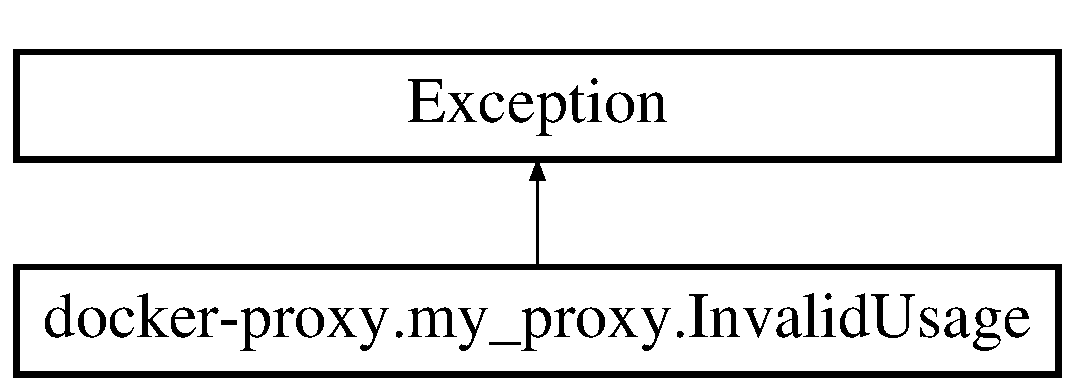
\includegraphics[height=2.000000cm]{classdocker-proxy_1_1my__proxy_1_1_invalid_usage}
\end{center}
\end{figure}
\subsection*{Public Member Functions}
\begin{DoxyCompactItemize}
\item 
\mbox{\Hypertarget{classdocker-proxy_1_1my__proxy_1_1_invalid_usage_aa785dfd5e9946eb87e2a94d4544bc656}\label{classdocker-proxy_1_1my__proxy_1_1_invalid_usage_aa785dfd5e9946eb87e2a94d4544bc656}} 
def {\bfseries \+\_\+\+\_\+init\+\_\+\+\_\+} (self, message, status\+\_\+code=None, payload=None)
\item 
\mbox{\Hypertarget{classdocker-proxy_1_1my__proxy_1_1_invalid_usage_a50b7849f7141fc1455ace3691a9417a7}\label{classdocker-proxy_1_1my__proxy_1_1_invalid_usage_a50b7849f7141fc1455ace3691a9417a7}} 
def {\bfseries to\+\_\+dict} (self)
\end{DoxyCompactItemize}
\subsection*{Public Attributes}
\begin{DoxyCompactItemize}
\item 
\mbox{\Hypertarget{classdocker-proxy_1_1my__proxy_1_1_invalid_usage_aa61d504376bb9479db82cb7d97c70011}\label{classdocker-proxy_1_1my__proxy_1_1_invalid_usage_aa61d504376bb9479db82cb7d97c70011}} 
{\bfseries message}
\item 
\mbox{\Hypertarget{classdocker-proxy_1_1my__proxy_1_1_invalid_usage_a6503499a33bc2de008fb69c03f453eec}\label{classdocker-proxy_1_1my__proxy_1_1_invalid_usage_a6503499a33bc2de008fb69c03f453eec}} 
{\bfseries status\+\_\+code}
\item 
\mbox{\Hypertarget{classdocker-proxy_1_1my__proxy_1_1_invalid_usage_a658b9343c56fde3e1753fe8ad1e1a158}\label{classdocker-proxy_1_1my__proxy_1_1_invalid_usage_a658b9343c56fde3e1753fe8ad1e1a158}} 
{\bfseries payload}
\end{DoxyCompactItemize}
\subsection*{Static Public Attributes}
\begin{DoxyCompactItemize}
\item 
\mbox{\Hypertarget{classdocker-proxy_1_1my__proxy_1_1_invalid_usage_aa06f3c7722ee51c93e799a0e57f67a32}\label{classdocker-proxy_1_1my__proxy_1_1_invalid_usage_aa06f3c7722ee51c93e799a0e57f67a32}} 
int {\bfseries status\+\_\+code} = 400
\end{DoxyCompactItemize}


\subsection{Detailed Description}
\begin{DoxyVerb}class to return specific return type codes
\end{DoxyVerb}
 

The documentation for this class was generated from the following file\+:\begin{DoxyCompactItemize}
\item 
my\+\_\+proxy.\+py\end{DoxyCompactItemize}

\hypertarget{classdocker-proxy_1_1unit__tests_1_1_md5_test}{}\section{docker-\/proxy.unit\+\_\+tests.\+Md5\+Test Class Reference}
\label{classdocker-proxy_1_1unit__tests_1_1_md5_test}\index{docker-\/proxy.\+unit\+\_\+tests.\+Md5\+Test@{docker-\/proxy.\+unit\+\_\+tests.\+Md5\+Test}}
Inheritance diagram for docker-\/proxy.unit\+\_\+tests.\+Md5\+Test\+:\begin{figure}[H]
\begin{center}
\leavevmode
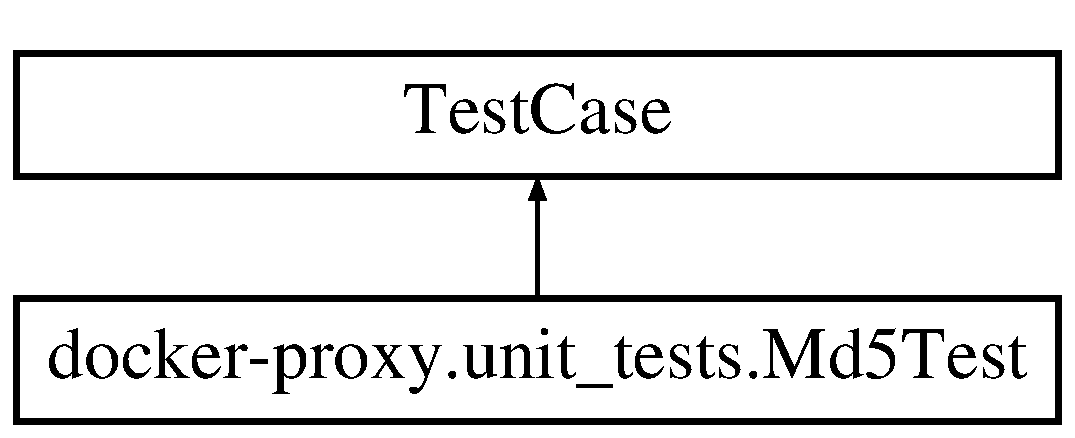
\includegraphics[height=2.000000cm]{classdocker-proxy_1_1unit__tests_1_1_md5_test}
\end{center}
\end{figure}
\subsection*{Public Member Functions}
\begin{DoxyCompactItemize}
\item 
def \mbox{\hyperlink{classdocker-proxy_1_1unit__tests_1_1_md5_test_a964cee9ecd446be83cdd9f50ff401203}{test\+\_\+is\+\_\+there\+\_\+config}} (self)
\item 
def \mbox{\hyperlink{classdocker-proxy_1_1unit__tests_1_1_md5_test_ac200f662c944e9c1f857de062fa6bd85}{test\+\_\+random\+\_\+port\+\_\+generator\+\_\+not\+\_\+restricred}} (self)
\item 
def \mbox{\hyperlink{classdocker-proxy_1_1unit__tests_1_1_md5_test_acc4c5dfd97e4925662798cd78a992772}{test\+\_\+random\+\_\+port\+\_\+generator\+\_\+is\+\_\+int}} (self)
\item 
def \mbox{\hyperlink{classdocker-proxy_1_1unit__tests_1_1_md5_test_a7a31a78746cfbad0c3d3a740f8ab50fd}{test\+\_\+random\+\_\+volume\+\_\+is\+\_\+string}} (self)
\end{DoxyCompactItemize}


\subsection{Member Function Documentation}
\mbox{\Hypertarget{classdocker-proxy_1_1unit__tests_1_1_md5_test_a964cee9ecd446be83cdd9f50ff401203}\label{classdocker-proxy_1_1unit__tests_1_1_md5_test_a964cee9ecd446be83cdd9f50ff401203}} 
\index{docker-\/proxy\+::unit\+\_\+tests\+::\+Md5\+Test@{docker-\/proxy\+::unit\+\_\+tests\+::\+Md5\+Test}!test\+\_\+is\+\_\+there\+\_\+config@{test\+\_\+is\+\_\+there\+\_\+config}}
\index{test\+\_\+is\+\_\+there\+\_\+config@{test\+\_\+is\+\_\+there\+\_\+config}!docker-\/proxy\+::unit\+\_\+tests\+::\+Md5\+Test@{docker-\/proxy\+::unit\+\_\+tests\+::\+Md5\+Test}}
\subsubsection{\texorpdfstring{test\+\_\+is\+\_\+there\+\_\+config()}{test\_is\_there\_config()}}
{\footnotesize\ttfamily def docker-\/proxy.\+unit\+\_\+tests.\+Md5\+Test.\+test\+\_\+is\+\_\+there\+\_\+config (\begin{DoxyParamCaption}\item[{}]{self }\end{DoxyParamCaption})}

\begin{DoxyVerb}Test if there is config file
:return:
\end{DoxyVerb}
 \mbox{\Hypertarget{classdocker-proxy_1_1unit__tests_1_1_md5_test_acc4c5dfd97e4925662798cd78a992772}\label{classdocker-proxy_1_1unit__tests_1_1_md5_test_acc4c5dfd97e4925662798cd78a992772}} 
\index{docker-\/proxy\+::unit\+\_\+tests\+::\+Md5\+Test@{docker-\/proxy\+::unit\+\_\+tests\+::\+Md5\+Test}!test\+\_\+random\+\_\+port\+\_\+generator\+\_\+is\+\_\+int@{test\+\_\+random\+\_\+port\+\_\+generator\+\_\+is\+\_\+int}}
\index{test\+\_\+random\+\_\+port\+\_\+generator\+\_\+is\+\_\+int@{test\+\_\+random\+\_\+port\+\_\+generator\+\_\+is\+\_\+int}!docker-\/proxy\+::unit\+\_\+tests\+::\+Md5\+Test@{docker-\/proxy\+::unit\+\_\+tests\+::\+Md5\+Test}}
\subsubsection{\texorpdfstring{test\+\_\+random\+\_\+port\+\_\+generator\+\_\+is\+\_\+int()}{test\_random\_port\_generator\_is\_int()}}
{\footnotesize\ttfamily def docker-\/proxy.\+unit\+\_\+tests.\+Md5\+Test.\+test\+\_\+random\+\_\+port\+\_\+generator\+\_\+is\+\_\+int (\begin{DoxyParamCaption}\item[{}]{self }\end{DoxyParamCaption})}

\begin{DoxyVerb}test if random port is generating an int
:return:
\end{DoxyVerb}
 \mbox{\Hypertarget{classdocker-proxy_1_1unit__tests_1_1_md5_test_ac200f662c944e9c1f857de062fa6bd85}\label{classdocker-proxy_1_1unit__tests_1_1_md5_test_ac200f662c944e9c1f857de062fa6bd85}} 
\index{docker-\/proxy\+::unit\+\_\+tests\+::\+Md5\+Test@{docker-\/proxy\+::unit\+\_\+tests\+::\+Md5\+Test}!test\+\_\+random\+\_\+port\+\_\+generator\+\_\+not\+\_\+restricred@{test\+\_\+random\+\_\+port\+\_\+generator\+\_\+not\+\_\+restricred}}
\index{test\+\_\+random\+\_\+port\+\_\+generator\+\_\+not\+\_\+restricred@{test\+\_\+random\+\_\+port\+\_\+generator\+\_\+not\+\_\+restricred}!docker-\/proxy\+::unit\+\_\+tests\+::\+Md5\+Test@{docker-\/proxy\+::unit\+\_\+tests\+::\+Md5\+Test}}
\subsubsection{\texorpdfstring{test\+\_\+random\+\_\+port\+\_\+generator\+\_\+not\+\_\+restricred()}{test\_random\_port\_generator\_not\_restricred()}}
{\footnotesize\ttfamily def docker-\/proxy.\+unit\+\_\+tests.\+Md5\+Test.\+test\+\_\+random\+\_\+port\+\_\+generator\+\_\+not\+\_\+restricred (\begin{DoxyParamCaption}\item[{}]{self }\end{DoxyParamCaption})}

\begin{DoxyVerb}Test if random generated port is not in restricted list
:return:
\end{DoxyVerb}
 \mbox{\Hypertarget{classdocker-proxy_1_1unit__tests_1_1_md5_test_a7a31a78746cfbad0c3d3a740f8ab50fd}\label{classdocker-proxy_1_1unit__tests_1_1_md5_test_a7a31a78746cfbad0c3d3a740f8ab50fd}} 
\index{docker-\/proxy\+::unit\+\_\+tests\+::\+Md5\+Test@{docker-\/proxy\+::unit\+\_\+tests\+::\+Md5\+Test}!test\+\_\+random\+\_\+volume\+\_\+is\+\_\+string@{test\+\_\+random\+\_\+volume\+\_\+is\+\_\+string}}
\index{test\+\_\+random\+\_\+volume\+\_\+is\+\_\+string@{test\+\_\+random\+\_\+volume\+\_\+is\+\_\+string}!docker-\/proxy\+::unit\+\_\+tests\+::\+Md5\+Test@{docker-\/proxy\+::unit\+\_\+tests\+::\+Md5\+Test}}
\subsubsection{\texorpdfstring{test\+\_\+random\+\_\+volume\+\_\+is\+\_\+string()}{test\_random\_volume\_is\_string()}}
{\footnotesize\ttfamily def docker-\/proxy.\+unit\+\_\+tests.\+Md5\+Test.\+test\+\_\+random\+\_\+volume\+\_\+is\+\_\+string (\begin{DoxyParamCaption}\item[{}]{self }\end{DoxyParamCaption})}

\begin{DoxyVerb}test of random volume name is str
:return:
\end{DoxyVerb}
 

The documentation for this class was generated from the following file\+:\begin{DoxyCompactItemize}
\item 
unit\+\_\+tests.\+py\end{DoxyCompactItemize}

\hypertarget{classdocker-proxy_1_1my__proxy_1_1_mount_points}{}\section{docker-\/proxy.my\+\_\+proxy.\+Mount\+Points Class Reference}
\label{classdocker-proxy_1_1my__proxy_1_1_mount_points}\index{docker-\/proxy.\+my\+\_\+proxy.\+Mount\+Points@{docker-\/proxy.\+my\+\_\+proxy.\+Mount\+Points}}
Inheritance diagram for docker-\/proxy.my\+\_\+proxy.\+Mount\+Points\+:\begin{figure}[H]
\begin{center}
\leavevmode
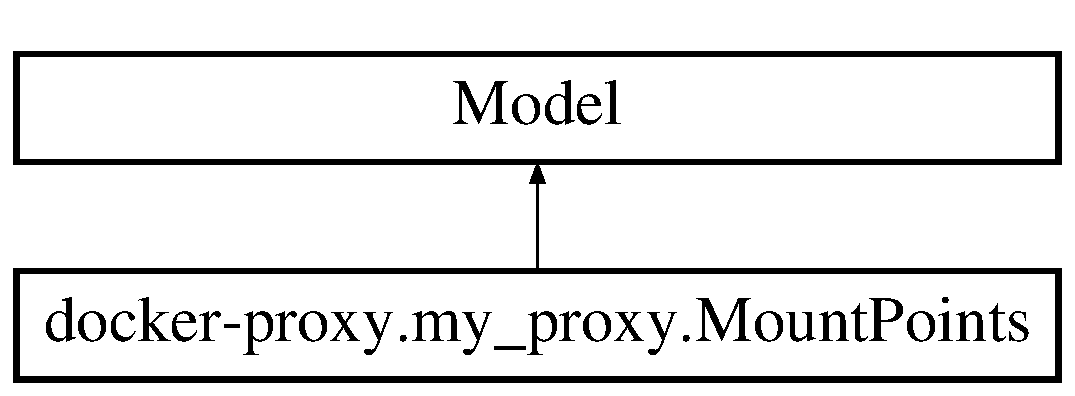
\includegraphics[height=2.000000cm]{classdocker-proxy_1_1my__proxy_1_1_mount_points}
\end{center}
\end{figure}
\subsection*{Public Member Functions}
\begin{DoxyCompactItemize}
\item 
def \hyperlink{classdocker-proxy_1_1my__proxy_1_1_mount_points_a559b6a122b5406dda695f40dc5eda8e9}{\+\_\+\+\_\+init\+\_\+\+\_\+} (self, \hyperlink{classdocker-proxy_1_1my__proxy_1_1_mount_points_aa49cde7530c0edaec96a4407707e714d}{owner}, \hyperlink{classdocker-proxy_1_1my__proxy_1_1_mount_points_aa7cfbe6eb066a60a4b6a0399fc64e003}{mount\+\_\+point}, \hyperlink{classdocker-proxy_1_1my__proxy_1_1_mount_points_aec1c878c659bd308f99b529d397d85c7}{volume\+\_\+name}, \hyperlink{classdocker-proxy_1_1my__proxy_1_1_mount_points_a6008b3f58ac2dd027f1d637cc84ee78c}{size\+\_\+plan})
\item 
def \hyperlink{classdocker-proxy_1_1my__proxy_1_1_mount_points_aea56d9596b2864b4d089b0f34744f3f4}{\+\_\+\+\_\+repr\+\_\+\+\_\+} (self)
\end{DoxyCompactItemize}
\subsection*{Static Public Attributes}
\begin{DoxyCompactItemize}
\item 
\hyperlink{classdocker-proxy_1_1my__proxy_1_1_mount_points_a17378df4d222e5d86f97d966e5ba30ee}{id} = db.\+Column(db.\+Integer, primary\+\_\+key=True, autoincrement=True)
\item 
\hyperlink{classdocker-proxy_1_1my__proxy_1_1_mount_points_aa49cde7530c0edaec96a4407707e714d}{owner} = db.\+Column(db.\+String(80), unique=True)
\item 
\hyperlink{classdocker-proxy_1_1my__proxy_1_1_mount_points_aa7cfbe6eb066a60a4b6a0399fc64e003}{mount\+\_\+point} = db.\+Column(db.\+String(200))
\item 
\hyperlink{classdocker-proxy_1_1my__proxy_1_1_mount_points_aec1c878c659bd308f99b529d397d85c7}{volume\+\_\+name} = db.\+Column(db.\+String(200))
\item 
\hyperlink{classdocker-proxy_1_1my__proxy_1_1_mount_points_a6008b3f58ac2dd027f1d637cc84ee78c}{size\+\_\+plan} = db.\+Column(db.\+String(80))
\end{DoxyCompactItemize}


\subsection{Detailed Description}
\begin{DoxyVerb}let's create the mount points table
\end{DoxyVerb}
 

Definition at line 73 of file my\+\_\+proxy.\+py.



\subsection{Constructor \& Destructor Documentation}
\hypertarget{classdocker-proxy_1_1my__proxy_1_1_mount_points_a559b6a122b5406dda695f40dc5eda8e9}{}\label{classdocker-proxy_1_1my__proxy_1_1_mount_points_a559b6a122b5406dda695f40dc5eda8e9} 
\index{docker-\/proxy\+::my\+\_\+proxy\+::\+Mount\+Points@{docker-\/proxy\+::my\+\_\+proxy\+::\+Mount\+Points}!\+\_\+\+\_\+init\+\_\+\+\_\+@{\+\_\+\+\_\+init\+\_\+\+\_\+}}
\index{\+\_\+\+\_\+init\+\_\+\+\_\+@{\+\_\+\+\_\+init\+\_\+\+\_\+}!docker-\/proxy\+::my\+\_\+proxy\+::\+Mount\+Points@{docker-\/proxy\+::my\+\_\+proxy\+::\+Mount\+Points}}
\subsubsection{\texorpdfstring{\+\_\+\+\_\+init\+\_\+\+\_\+()}{\_\_init\_\_()}}
{\footnotesize\ttfamily def docker-\/proxy.\+my\+\_\+proxy.\+Mount\+Points.\+\_\+\+\_\+init\+\_\+\+\_\+ (\begin{DoxyParamCaption}\item[{}]{self,  }\item[{}]{owner,  }\item[{}]{mount\+\_\+point,  }\item[{}]{volume\+\_\+name,  }\item[{}]{size\+\_\+plan }\end{DoxyParamCaption})}



Definition at line 84 of file my\+\_\+proxy.\+py.



\subsection{Member Function Documentation}
\hypertarget{classdocker-proxy_1_1my__proxy_1_1_mount_points_aea56d9596b2864b4d089b0f34744f3f4}{}\label{classdocker-proxy_1_1my__proxy_1_1_mount_points_aea56d9596b2864b4d089b0f34744f3f4} 
\index{docker-\/proxy\+::my\+\_\+proxy\+::\+Mount\+Points@{docker-\/proxy\+::my\+\_\+proxy\+::\+Mount\+Points}!\+\_\+\+\_\+repr\+\_\+\+\_\+@{\+\_\+\+\_\+repr\+\_\+\+\_\+}}
\index{\+\_\+\+\_\+repr\+\_\+\+\_\+@{\+\_\+\+\_\+repr\+\_\+\+\_\+}!docker-\/proxy\+::my\+\_\+proxy\+::\+Mount\+Points@{docker-\/proxy\+::my\+\_\+proxy\+::\+Mount\+Points}}
\subsubsection{\texorpdfstring{\+\_\+\+\_\+repr\+\_\+\+\_\+()}{\_\_repr\_\_()}}
{\footnotesize\ttfamily def docker-\/proxy.\+my\+\_\+proxy.\+Mount\+Points.\+\_\+\+\_\+repr\+\_\+\+\_\+ (\begin{DoxyParamCaption}\item[{}]{self }\end{DoxyParamCaption})}

\begin{DoxyVerb}return only the mount point
\end{DoxyVerb}
 

Definition at line 90 of file my\+\_\+proxy.\+py.



\subsection{Member Data Documentation}
\hypertarget{classdocker-proxy_1_1my__proxy_1_1_mount_points_a17378df4d222e5d86f97d966e5ba30ee}{}\label{classdocker-proxy_1_1my__proxy_1_1_mount_points_a17378df4d222e5d86f97d966e5ba30ee} 
\index{docker-\/proxy\+::my\+\_\+proxy\+::\+Mount\+Points@{docker-\/proxy\+::my\+\_\+proxy\+::\+Mount\+Points}!id@{id}}
\index{id@{id}!docker-\/proxy\+::my\+\_\+proxy\+::\+Mount\+Points@{docker-\/proxy\+::my\+\_\+proxy\+::\+Mount\+Points}}
\subsubsection{\texorpdfstring{id}{id}}
{\footnotesize\ttfamily docker-\/proxy.\+my\+\_\+proxy.\+Mount\+Points.\+id = db.\+Column(db.\+Integer, primary\+\_\+key=True, autoincrement=True)\hspace{0.3cm}{\ttfamily [static]}}



Definition at line 78 of file my\+\_\+proxy.\+py.

\hypertarget{classdocker-proxy_1_1my__proxy_1_1_mount_points_aa7cfbe6eb066a60a4b6a0399fc64e003}{}\label{classdocker-proxy_1_1my__proxy_1_1_mount_points_aa7cfbe6eb066a60a4b6a0399fc64e003} 
\index{docker-\/proxy\+::my\+\_\+proxy\+::\+Mount\+Points@{docker-\/proxy\+::my\+\_\+proxy\+::\+Mount\+Points}!mount\+\_\+point@{mount\+\_\+point}}
\index{mount\+\_\+point@{mount\+\_\+point}!docker-\/proxy\+::my\+\_\+proxy\+::\+Mount\+Points@{docker-\/proxy\+::my\+\_\+proxy\+::\+Mount\+Points}}
\subsubsection{\texorpdfstring{mount\+\_\+point}{mount\_point}}
{\footnotesize\ttfamily docker-\/proxy.\+my\+\_\+proxy.\+Mount\+Points.\+mount\+\_\+point = db.\+Column(db.\+String(200))\hspace{0.3cm}{\ttfamily [static]}}



Definition at line 80 of file my\+\_\+proxy.\+py.

\hypertarget{classdocker-proxy_1_1my__proxy_1_1_mount_points_aa49cde7530c0edaec96a4407707e714d}{}\label{classdocker-proxy_1_1my__proxy_1_1_mount_points_aa49cde7530c0edaec96a4407707e714d} 
\index{docker-\/proxy\+::my\+\_\+proxy\+::\+Mount\+Points@{docker-\/proxy\+::my\+\_\+proxy\+::\+Mount\+Points}!owner@{owner}}
\index{owner@{owner}!docker-\/proxy\+::my\+\_\+proxy\+::\+Mount\+Points@{docker-\/proxy\+::my\+\_\+proxy\+::\+Mount\+Points}}
\subsubsection{\texorpdfstring{owner}{owner}}
{\footnotesize\ttfamily docker-\/proxy.\+my\+\_\+proxy.\+Mount\+Points.\+owner = db.\+Column(db.\+String(80), unique=True)\hspace{0.3cm}{\ttfamily [static]}}



Definition at line 79 of file my\+\_\+proxy.\+py.

\hypertarget{classdocker-proxy_1_1my__proxy_1_1_mount_points_a6008b3f58ac2dd027f1d637cc84ee78c}{}\label{classdocker-proxy_1_1my__proxy_1_1_mount_points_a6008b3f58ac2dd027f1d637cc84ee78c} 
\index{docker-\/proxy\+::my\+\_\+proxy\+::\+Mount\+Points@{docker-\/proxy\+::my\+\_\+proxy\+::\+Mount\+Points}!size\+\_\+plan@{size\+\_\+plan}}
\index{size\+\_\+plan@{size\+\_\+plan}!docker-\/proxy\+::my\+\_\+proxy\+::\+Mount\+Points@{docker-\/proxy\+::my\+\_\+proxy\+::\+Mount\+Points}}
\subsubsection{\texorpdfstring{size\+\_\+plan}{size\_plan}}
{\footnotesize\ttfamily docker-\/proxy.\+my\+\_\+proxy.\+Mount\+Points.\+size\+\_\+plan = db.\+Column(db.\+String(80))\hspace{0.3cm}{\ttfamily [static]}}



Definition at line 82 of file my\+\_\+proxy.\+py.

\hypertarget{classdocker-proxy_1_1my__proxy_1_1_mount_points_aec1c878c659bd308f99b529d397d85c7}{}\label{classdocker-proxy_1_1my__proxy_1_1_mount_points_aec1c878c659bd308f99b529d397d85c7} 
\index{docker-\/proxy\+::my\+\_\+proxy\+::\+Mount\+Points@{docker-\/proxy\+::my\+\_\+proxy\+::\+Mount\+Points}!volume\+\_\+name@{volume\+\_\+name}}
\index{volume\+\_\+name@{volume\+\_\+name}!docker-\/proxy\+::my\+\_\+proxy\+::\+Mount\+Points@{docker-\/proxy\+::my\+\_\+proxy\+::\+Mount\+Points}}
\subsubsection{\texorpdfstring{volume\+\_\+name}{volume\_name}}
{\footnotesize\ttfamily docker-\/proxy.\+my\+\_\+proxy.\+Mount\+Points.\+volume\+\_\+name = db.\+Column(db.\+String(200))\hspace{0.3cm}{\ttfamily [static]}}



Definition at line 81 of file my\+\_\+proxy.\+py.



The documentation for this class was generated from the following file\+:\begin{DoxyCompactItemize}
\item 
\hyperlink{my__proxy_8py}{my\+\_\+proxy.\+py}\end{DoxyCompactItemize}

\chapter{File Documentation}
\hypertarget{____init_____8py}{}\section{\+\_\+\+\_\+init\+\_\+\+\_\+.\+py File Reference}
\label{____init_____8py}\index{\+\_\+\+\_\+init\+\_\+\+\_\+.\+py@{\+\_\+\+\_\+init\+\_\+\+\_\+.\+py}}
\subsection*{Namespaces}
\begin{DoxyCompactItemize}
\item 
 \hyperlink{namespacedocker-proxy}{docker-\/proxy}
\end{DoxyCompactItemize}
\subsection*{Variables}
\begin{DoxyCompactItemize}
\item 
\hyperlink{namespacedocker-proxy_a77b1cf15d8b7127338d8596c99d67ed7}{docker-\/proxy.\+app} = Flask(\+\_\+\+\_\+name\+\_\+\+\_\+)
\end{DoxyCompactItemize}

\hypertarget{config__parser_8py}{}\section{config\+\_\+parser.\+py File Reference}
\label{config__parser_8py}\index{config\+\_\+parser.\+py@{config\+\_\+parser.\+py}}
\subsection*{Namespaces}
\begin{DoxyCompactItemize}
\item 
 \hyperlink{namespacedocker-proxy_1_1config__parser}{docker-\/proxy.\+config\+\_\+parser}
\end{DoxyCompactItemize}
\subsection*{Functions}
\begin{DoxyCompactItemize}
\item 
def \hyperlink{namespacedocker-proxy_1_1config__parser_aa9dfa23e3cb83a9b109517727216624a}{docker-\/proxy.\+config\+\_\+parser.\+check\+\_\+if\+\_\+config\+\_\+exists} (config\+\_\+file)
\item 
def \hyperlink{namespacedocker-proxy_1_1config__parser_a52b3461dc4ed5a410f566197208b4b13}{docker-\/proxy.\+config\+\_\+parser.\+config\+\_\+params} (section)
\end{DoxyCompactItemize}

\hypertarget{connect__docker__server_8py}{}\section{connect\+\_\+docker\+\_\+server.\+py File Reference}
\label{connect__docker__server_8py}\index{connect\+\_\+docker\+\_\+server.\+py@{connect\+\_\+docker\+\_\+server.\+py}}
\subsection*{Namespaces}
\begin{DoxyCompactItemize}
\item 
 \hyperlink{namespacedocker-proxy_1_1connect__docker__server}{docker-\/proxy.\+connect\+\_\+docker\+\_\+server}
\end{DoxyCompactItemize}
\subsection*{Functions}
\begin{DoxyCompactItemize}
\item 
def \hyperlink{namespacedocker-proxy_1_1connect__docker__server_a5a405d25b986678755c9a1aedeb066f8}{docker-\/proxy.\+connect\+\_\+docker\+\_\+server.\+connect\+\_\+docker\+\_\+server} ()
\end{DoxyCompactItemize}
\subsection*{Variables}
\begin{DoxyCompactItemize}
\item 
def \hyperlink{namespacedocker-proxy_1_1connect__docker__server_aa7f3f87149d03ba3fd92b1b60a011454}{docker-\/proxy.\+connect\+\_\+docker\+\_\+server.\+connect} = connect\+\_\+docker\+\_\+server()
\end{DoxyCompactItemize}

\hypertarget{models_8py}{}\section{models.\+py File Reference}
\label{models_8py}\index{models.\+py@{models.\+py}}
\subsection*{Classes}
\begin{DoxyCompactItemize}
\item 
class \hyperlink{classdocker-proxy_1_1models_1_1_container_names}{docker-\/proxy.\+models.\+Container\+Names}
\end{DoxyCompactItemize}
\subsection*{Namespaces}
\begin{DoxyCompactItemize}
\item 
 \hyperlink{namespacedocker-proxy_1_1models}{docker-\/proxy.\+models}
\end{DoxyCompactItemize}
\subsection*{Variables}
\begin{DoxyCompactItemize}
\item 
\hyperlink{namespacedocker-proxy_1_1models_a6d8a79afafa0fb31efaeda3e08b9a31d}{docker-\/proxy.\+models.\+db} = S\+Q\+L\+Alchemy()
\end{DoxyCompactItemize}

\hypertarget{my__proxy_8py}{}\section{my\+\_\+proxy.\+py File Reference}
\label{my__proxy_8py}\index{my\+\_\+proxy.\+py@{my\+\_\+proxy.\+py}}
\subsection*{Classes}
\begin{DoxyCompactItemize}
\item 
class \hyperlink{classdocker-proxy_1_1my__proxy_1_1_invalid_usage}{docker-\/proxy.\+my\+\_\+proxy.\+Invalid\+Usage}
\item 
class \hyperlink{classdocker-proxy_1_1my__proxy_1_1_mount_points}{docker-\/proxy.\+my\+\_\+proxy.\+Mount\+Points}
\item 
class \hyperlink{classdocker-proxy_1_1my__proxy_1_1_container_names}{docker-\/proxy.\+my\+\_\+proxy.\+Container\+Names}
\end{DoxyCompactItemize}
\subsection*{Namespaces}
\begin{DoxyCompactItemize}
\item 
 \hyperlink{namespacedocker-proxy_1_1my__proxy}{docker-\/proxy.\+my\+\_\+proxy}
\end{DoxyCompactItemize}
\subsection*{Functions}
\begin{DoxyCompactItemize}
\item 
def \hyperlink{namespacedocker-proxy_1_1my__proxy_a0c927506d8346f17b620ac8e131174d0}{docker-\/proxy.\+my\+\_\+proxy.\+handle\+\_\+invalid\+\_\+usage} (error)
\item 
def \hyperlink{namespacedocker-proxy_1_1my__proxy_a219b29b5c79ad35297fb1f1deef275a3}{docker-\/proxy.\+my\+\_\+proxy.\+require\+\_\+appkey} (view\+\_\+function)
\item 
def \hyperlink{namespacedocker-proxy_1_1my__proxy_a0bf8985afda99ee825115bd5df0b6b40}{docker-\/proxy.\+my\+\_\+proxy.\+give\+\_\+me\+\_\+something\+\_\+unique} (name\+\_\+of\+\_\+container, hostname, owner, password, service\+\_\+name)
\item 
def \hyperlink{namespacedocker-proxy_1_1my__proxy_a32ea0c997fb4530822b84a6861f9666c}{docker-\/proxy.\+my\+\_\+proxy.\+give\+\_\+me\+\_\+mount\+\_\+point} (owner, size\+\_\+plan)
\item 
def \hyperlink{namespacedocker-proxy_1_1my__proxy_a7c16c9ad1dd493bd800fb0ccb04cfe32}{docker-\/proxy.\+my\+\_\+proxy.\+docker\+\_\+create} (name\+\_\+id, username, password, service, diskspace, image\+\_\+name, internal\+\_\+port, exec\+\_\+this)
\item 
def \hyperlink{namespacedocker-proxy_1_1my__proxy_a5c4e8ad5904fc41dc6e53312834445ae}{docker-\/proxy.\+my\+\_\+proxy.\+storage\+\_\+sum} ()
\item 
def \hyperlink{namespacedocker-proxy_1_1my__proxy_a2d2a47f5b69859690e7d948cbe5898a4}{docker-\/proxy.\+my\+\_\+proxy.\+storage} ()
\item 
def \hyperlink{namespacedocker-proxy_1_1my__proxy_ae108a533f8a3353f199f69883994c3cf}{docker-\/proxy.\+my\+\_\+proxy.\+stasts} (container\+\_\+id)
\item 
def \hyperlink{namespacedocker-proxy_1_1my__proxy_a96423469e4fe05cd336a8af7cb28d2ba}{docker-\/proxy.\+my\+\_\+proxy.\+management} (container\+\_\+id)
\item 
def \hyperlink{namespacedocker-proxy_1_1my__proxy_abf1a0936dc4dd14a5aaa78854c6583ce}{docker-\/proxy.\+my\+\_\+proxy.\+executecommands} (name\+\_\+id)
\item 
def \hyperlink{namespacedocker-proxy_1_1my__proxy_aaab4affe92f8974338caa10c0cf70c22}{docker-\/proxy.\+my\+\_\+proxy.\+makevm} (name\+\_\+id)
\item 
def \hyperlink{namespacedocker-proxy_1_1my__proxy_ad3276ec211f2fe107e03e4ed5e346df6}{docker-\/proxy.\+my\+\_\+proxy.\+version} ()
\item 
def \hyperlink{namespacedocker-proxy_1_1my__proxy_a7f6173c933a3e2e679eedb795386a08e}{docker-\/proxy.\+my\+\_\+proxy.\+query} (name)
\item 
def \hyperlink{namespacedocker-proxy_1_1my__proxy_a51d957f776d16e54de05b7034b113c1f}{docker-\/proxy.\+my\+\_\+proxy.\+investigate} (container\+\_\+id)
\item 
def \hyperlink{namespacedocker-proxy_1_1my__proxy_a84a1e1b9285c530fcd8b04177d08cdb3}{docker-\/proxy.\+my\+\_\+proxy.\+showstuff} ()
\end{DoxyCompactItemize}
\subsection*{Variables}
\begin{DoxyCompactItemize}
\item 
\hyperlink{namespacedocker-proxy_1_1my__proxy_a1316b64a06ccf8940bd886efa8d18660}{docker-\/proxy.\+my\+\_\+proxy.\+app} = Flask(\+\_\+\+\_\+name\+\_\+\+\_\+)
\item 
\hyperlink{namespacedocker-proxy_1_1my__proxy_a3cda0544280d27f01985434ab3efa4b3}{docker-\/proxy.\+my\+\_\+proxy.\+db} = S\+Q\+L\+Alchemy(app)
\item 
\hyperlink{namespacedocker-proxy_1_1my__proxy_a4cb4fb47e79c0c24a5b66136731a0b0c}{docker-\/proxy.\+my\+\_\+proxy.\+debug}
\end{DoxyCompactItemize}

\hypertarget{_r_e_a_d_m_e_8md}{}\section{R\+E\+A\+D\+M\+E.\+md File Reference}
\label{_r_e_a_d_m_e_8md}\index{R\+E\+A\+D\+M\+E.\+md@{R\+E\+A\+D\+M\+E.\+md}}

\hypertarget{unit__tests_8py}{}\section{unit\+\_\+tests.\+py File Reference}
\label{unit__tests_8py}\index{unit\+\_\+tests.\+py@{unit\+\_\+tests.\+py}}
\subsection*{Classes}
\begin{DoxyCompactItemize}
\item 
class \hyperlink{classdocker-proxy_1_1unit__tests_1_1_md5_test}{docker-\/proxy.\+unit\+\_\+tests.\+Md5\+Test}
\end{DoxyCompactItemize}
\subsection*{Namespaces}
\begin{DoxyCompactItemize}
\item 
 \hyperlink{namespacedocker-proxy_1_1unit__tests}{docker-\/proxy.\+unit\+\_\+tests}
\end{DoxyCompactItemize}

\hypertarget{validate__hostname_8py}{}\section{validate\+\_\+hostname.\+py File Reference}
\label{validate__hostname_8py}\index{validate\+\_\+hostname.\+py@{validate\+\_\+hostname.\+py}}
\subsection*{Namespaces}
\begin{DoxyCompactItemize}
\item 
 \hyperlink{namespacedocker-proxy_1_1validate__hostname}{docker-\/proxy.\+validate\+\_\+hostname}
\end{DoxyCompactItemize}
\subsection*{Functions}
\begin{DoxyCompactItemize}
\item 
def \hyperlink{namespacedocker-proxy_1_1validate__hostname_a78870bf36758d0abb57f63eea91fd8b7}{docker-\/proxy.\+validate\+\_\+hostname.\+isvalidhostname} (hostname)
\end{DoxyCompactItemize}

%--- End generated contents ---

% Index
\backmatter
\newpage
\phantomsection
\clearemptydoublepage
\addcontentsline{toc}{chapter}{Index}
\printindex

\end{document}
